\documentclass{article}
\usepackage[a4paper, margin=0.5in]{geometry}
\usepackage{amsmath}
\usepackage{amssymb}
\usepackage{physics}
\usepackage{tikz}
\usepackage[american]{circuitikz}
\usepackage{physoly}
\usepackage{siunitx}
\usepackage{bbm}

\usepackage{pgfplots}
\pgfplotsset{compat=1.16} 

\begin{document}
\tableofcontents
\section{What is an Electric Circuit}
\begin{definition}
    An electric circuit is an interconnection of circuit elements (incl. Conductors, semi-conductors, non-conductors). 
\end{definition}

\section{Electrical Variables}
    To help us analyze electric circuits, we define several electrical variables:
    \subsection{Current}
    \begin{definition}
        Electric currents: The "movement" or rate of change of electrical charge. 
        \begin{equation}
            i\equiv\frac{dq}{dt}
        \end{equation} 
        
        \begin{enumerate}
            \item S.I. unit: Ampere = Columb per second.
            \item The current has a direction, and its direction is defined as the direction of positive charge. (Can be shown with $\leftarrow$ or $\rightarrow$)
        \end{enumerate}
    \end{definition}
    \begin{itemize}
        \item When performing circuit analysis, the direction of positive current is either given or we are required to guess a direction of positive current and verify it later. 
        \item A positive current means the direction you guessed is correct. A negative current means the actual direction is the direction opposiing the current.
    \end{itemize}
    \subsection{Voltage}
    \begin{definition}
        Voltage: The energy required for 1C of charge between point A and B in a circuit is called the voltage between points A and B. 
        \begin{equation}
            V\equiv\frac{dw}{dq}
        \end{equation} 
        \begin{enumerate}
            \item S.I. unit: Volt = Joule per columb.
            \item The voltage also have polarity ($+$ or $-$). Positive polarity means energy is consumed when the charge moves from A to B.
        \end{enumerate}
    \end{definition}
    \begin{itemize}
        \item If the polarity is not given, guess a polarity 
        \item a positive voltage indicates the guess is correct and a negative voltage indicates the guess is incorrect.
    \end{itemize}
    \subsection{Power}
    \begin{definition}
        Power: The rate of delivering or absorbing energy.
        \begin{equation}
            p\equiv\frac{dw}{dt}
        \end{equation}
        \begin{enumerate}
            \item S.I. unit: Watt = Joule per second.
            \item Using chain rule, 
            \begin{equation}
                p=\frac{dw}{dt}=\frac{dw}{dq}\frac{dq}{dt}=iv
            \end{equation}
        \end{enumerate}
    \end{definition}
    \begin{itemize}
        \item \textbf{Note:} When a problem asks for a current or voltage, the direction/polarity \textbf{must} be indicated otherwise full credit will not be given.
    \end{itemize}
    \begin{definition}
        For a pair of v and i, PSC holds if the current direction \textbf{enters} the positive side of voltage polarity. If PSC holds, $p=+vi$; else $p=-vi$ 
        \begin{center}
            \begin{circuitikz}
                \draw (0,0) to[generic,o-o](5,0);
                \draw (7,0) to[generic,o-o](12,0);
                \draw (1.5,0.2) node{$+$};
                \draw (3.5,0.2) node{$-$};
                \draw (8.5,0.2) node{$+$};
                \draw (10.5,0.2) node{$-$};
                \draw[-latex](0.5,0)--(1,0)node[below]{$i_1$};
                \draw[-latex](8.5,0)--(8,0)node[below]{$i_2$};
            \end{circuitikz}
        \end{center}
        PSC holds on the left and does not hold on the right.
    \end{definition}
    \begin{itemize}
        \item The consequences of this convention are
        \begin{enumerate}
            \item $p>0\implies$power is absorbed
            \item $p<0\implies$power is delivered (generated by the circuit element)
        \end{enumerate}
    \end{itemize}
    \subsection{Examples}
    \begin{example}[1]
        Identify the devices that generate power in the circuit below and find the unknowns in the table.
        \begin{center}
            \begin{circuitikz}
                \draw 
                (0,0) to[generic,V=$v_1$] (0,4) 
                to[generic,V=$v_3$] (6,4);
                \draw
                (0,0) to (6,0)
                to[generic,V=$v_4$] (6,4);
                \draw
                (6,0) to (12,0) 
                to[generic,V=$v_5$] (12,4)
                to (6,4);
                \draw
                (0,4) to[generic,V=$v_2$] (6,0);
            \end{circuitikz}
        \end{center}
    \end{example}
    \begin{theorem}
        \textbf{Conservation of Power} states that the algebraic sum of the power of all elements in a circuit is zero. (algebraic means the signs are preserved)
        \begin{equation}
            \sum p=0
        \end{equation}
        \begin{prooof}
            Will not be presented at this point in the course.
        \end{prooof}
    \end{theorem}
    \begin{example}[2]
        \begin{center}
            \begin{circuitikz}
                \draw
                (0,0)node[anchor=east]{Cir.1} to[generic,o-o] (8,0)node[anchor=west]{Cir.2};
                \draw[-latex] (1,0)--(2,0) node[below]{i(t)};
            \end{circuitikz}
        \end{center}
        Given the above circuit and
        \begin{align}
            v(t)&=50(1-e^{-5000t})\text{V}\\
            i(t)&=10e^{-5000t}\text{A}
        \end{align}
        Find the total energy transfered to this device after $t=0$.
    \end{example}
    \begin{sol}[2]
        PSC holds. Thus,
        \begin{align}
            p(t)&=v(t)i(t)\\
            p(t)&=50(1-e^{-5000t})10(e^{-5000t})\text{W}
        \end{align}
        From the definition of power,
        \begin{align}
            p(t)&=\frac{dw}{dt}\therefore dw=p(t)dt\\
            w&=\int_0^\infty p(t)\dd t=\int_0^\infty 50(1-e^{-5000t})10(e^{-5000t}) \dd t=\frac{1}{20}\text{J}=50\text{mJ}
        \end{align}
    \end{sol}
\section{Circuit Elements}
    \subsection{Independent sources}
    \begin{enumerate}
        \item \textit{Independent voltage sources:} A circuit element that has a specific voltage independent of the current that flows through it.
        \begin{itemize}
            \item For example, the voltage can be a fixed voltage like $v_s=2$V or a variable voltage source like $v_s=2\sin(50t+2)$.
            \item On diagrams, generic voltage source is shown on the left and fixed (DC) voltage sources is shown on the right. For DC sources, the uppercase letter $V$ is commonly used.
            \begin{center}
                \begin{circuitikz}
                    \draw
                    (0,0)to[generic,V=,o-o](4,0);
                    \draw
                    (6,0)node[below]{$+$} to[battery,o-o](10,0)node[below]{$-$};    
                \end{circuitikz}
            \end{center}
            \item For DC source, the longer lines denotes positive voltage polarity and shorter lines denote negative voltage polarity.
            \item An sinsudal voltage is drawn as
            \begin{center}
                \begin{circuitikz}
                    \draw
                    (0,0)to[sinusoidal voltage source,V=,o-o](6,0);
                \end{circuitikz}
            \end{center}
            \item Questions
            \begin{enumerate}
                \item What is the direction of $i$ for the following voltage source?
                \begin{center}
                    \begin{circuitikz}
                        \draw
                        (0,0)to[generic,V=2V,o-o](6,0);
                    \end{circuitikz}
                \end{center}
                Answer: You cannot determine.
                \item Does a voltage source always generate power?
                
                Answer: No. Take the voltage source above. Take a current $i_1=2\text{A}\rightarrow$. Then, PSC holds and $p=vi=(2\text{V})(2\text{A})=4\text{W}$. Since $p>0$, the voltage source absorbs power.
            \end{enumerate}
        \end{itemize}

        \item \textit{Independent current source:} It gives a specific current independent of the voltage across it. Can be constant like $i_s=5$A or time dependent like $i_s=10\cos(15t)$
        
        \begin{itemize}
            \item The independent current source is drawn as
            \begin{center}
                \begin{circuitikz}
                    \draw
                    (0,0)to[I](6,0);
                \end{circuitikz}
            \end{center}
            \item Questions
            \begin{enumerate}
                \item What is the polarity of voltage across a current source?
                \item Does a current source always generate power?
            \end{enumerate}
            \item Do \textbf{not} let the word \textit{source} decieve you. A source is not associated with generating power.
        \end{itemize}
    \end{enumerate}
    \subsection{Dependent Sources}
    \begin{enumerate}
        \item \textit{Voltage-dependent voltage source:}
        \begin{center}
            \begin{circuitikz}
                \draw
                (0,0)to[cV,cV=$Kv_x$,o-o](6,0);
            \end{circuitikz}
        \end{center}
        The voltage of this source depends on voltages somewhere else in the circuit. i.e. $v_s=Kv_s$
        
        \item \textit{Current-dependent voltage source:}
        \begin{center}
            \begin{circuitikz}
                \draw
                (0,0)to[cI,cI=$Ki_x$,o-o](6,0);
            \end{circuitikz}
        \end{center}
        The voltage of this source depends on the current somewhere else in a circuit i.e. $v_s=k i_x$. Note k has the dimensions Current/Voltage.
        \item \textit{Voltage-dependent current source:}
        \item \textit{Current-dependent current source:}
    \end{enumerate}
    \subsection{Resistor}
    A resistor is a circuit element that keeps the ratio between the voltage and current constant.
    \begin{equation}
        R\equiv\frac{v}{i}
    \end{equation}
    \begin{itemize}
        \item S.I. unit: Volt per Amp or Ohm ($\Omega$).
        \item The resistor is drawn like this. If PSC holds, $v=Ri$ else $v=-Ri$. This is also known as Ohm's Law.
        \begin{center}
            \begin{circuitikz}
                \draw
                (0,0)to[R](6,0);
            \end{circuitikz}
        \end{center}
        \item The inverse of the resistence $R$ is called the conductance $G$
        \begin{equation}
            G\equiv\frac{1}{R}=\pm\frac{i}{v}
        \end{equation}
        \item The S.I. unit for conductance is 1/Ohm, also refered to as "mho" or "siemens" (Si).
        \item We could not find a generic relation for the power of a source, since $P=vi$ (assuming PSC holds). Since for a independent voltage source, we don't know the current and vise versa. For a resistor however, assume PSC holds,
        \begin{align}
            P=vi&=(Ri)i=Ri^2\\
            &=v\left(\frac{v}{R}\right)=\frac{v^2}{R}
        \end{align}
        If PSC doesn't hold,
        \begin{align}
            P=-vi&=-(-Ri)i=Ri^2\\
            &=-v\left(-\frac{v}{R}\right)=\frac{v^2}{R}
        \end{align}
        Thus, the power of a resistor is independent of whether or not PSC holds. For physical resistors, $R>0$ hence $P>0$ which means power is always absorbed.
    \end{itemize} 
    \subsection{Short Circuit} 
    A short circuit is the limiting behavior for a resistor as $R\to0$. Since $v=Ri$, the voltage is zero independent of the current. This is denoted with a solid line:
    \begin{center}
        \begin{circuitikz}
            \draw (0,0)to(6,0);
        \end{circuitikz}
    \end{center}
    \begin{itemize}
        \item Other names include zero ohm path or ideal conductor.
        \item \textbf{
            In analysis, all parts of a circuit that are connected using ideal conductor can be considered the same point in the circuit.
            }
    \end{itemize}
    \subsection{Open Circuit}
    The limiting behavior for a resistor as $R\to\infty$. Since $v=Ri$, the current is zero independent of the voltage. 
    \begin{center}
        \begin{circuitikz}
            \draw (0,0)to(2,0)to[open](4,0)to(6,0);
        \end{circuitikz}
    \end{center}
    For example, the air between the ground and transmission line can be treated like a open circuit, since air is not a conductor.

\section{Circuit Analysis Definitions}
\begin{definition}
    A \textbf{Node} is a junction of two or more circuit elements.
    \begin{center}
        \begin{circuitikz}
            \draw (0,0)to[V=$v_s$,-*](0,3);
            \draw (0,3)to[R=$R_2$,-*](4,3)to[R=$R_4$,-*](8,3)to[R=$R_5$](8,0)to(0,0);
            \draw (4,3)to[R=$R_3$](4,0);
            \draw (0,3)to[R=$R_1$,-*](4,0);
        \end{circuitikz}
    \end{center}
    The labelled points are nodes: top-left connects $v_s$, $R_1$ and $R_2$; top-center connects $R_2$, $R_3$, and $R_4$; top-right connects $R_4$ and $R_5$; as well as the region at the bottom (that are connected by short circuit as the junction of $v_s$, $R_1$, $R_3$, $R_5$).
\end{definition}
\begin{definition}
    Start moving from one node towards the other nodes. As long as no node is passed (\textbf{unless} it is a loop when start and end nodes are the same) more than once, the set of nodes passed is called a \textbf{Path}. 
    \begin{center}
        \begin{circuitikz}
            \draw (0,0)to[V=$v_s$,-*](0,3)node[left]{$N_1$};
            \draw (0,3)to[R=$R_2$,-*](4,3)to[R=$R_4$,-*](8,3)to[R=$R_5$](8,0)to(0,0);
            \draw (4,3)to[R=$R_3$](4,0);
            \draw (0,3)to[R=$R_1$,-*](4,0);
            \draw[-latex,blue](0,4)--(4,4)--(9,4)--(9,-1)--(4,-1);
            \draw[-latex,red](0,3.6)--(4,3.6)--(8.6,3.6)--(8.6,-0.4)--(4,-0.4)--(4,4);
        \end{circuitikz}
    \end{center}
    The blue one is a path, the red one is not.
\end{definition}
\begin{definition}
    If the beginning and end of a path is one node, that path is a \textbf{loop}.
    \begin{center}
        \begin{circuitikz}
            \draw (0,0)to[V=$v_s$,-*](0,3)node[left]{$N_1$};
            \draw (0,3)to[R=$R_2$,-*](4,3)to[R=$R_4$,-*](8,3)to[R=$R_5$](8,0)to(0,0);
            \draw (4,3)to[R=$R_3$](4,0);
            \draw (0,3)to[R=$R_1$,-*](4,0);
            \draw[-latex,blue](0,4)--(4,4)--(9,4)--(9,-1)--(4,-1)--(0,2);
            \draw[-latex,red](0,3.6)--(4,3.6)--(8.6,3.6)--(8.6,-0.4)--(4.2,-0.4)--(4.2,4);
        \end{circuitikz}
    \end{center}
    The blue one is a loop, the red one is not a loop.
\end{definition}
\subsection{Examples}
\begin{example}[1]
    Identify the loops in the circuit above circuit
\end{example}
\begin{sol}[1]
    Arrows are too hard to draw
    \begin{center}
        \begin{circuitikz}
            \draw (0,0)to[V=$v_s$,-*](0,3)node[left]{$N_1$};
            \draw (0,3)to[R=$R_2$,-*](4,3)to[R=$R_4$,-*](8,3)to[R=$R_5$](8,0)to(0,0);
            \draw (4,3)to[R=$R_3$](4,0);
            \draw (0,3)to[R=$R_1$,-*](4,0);
            \draw[-latex,blue](0,3.1)--(4,3.1)--(9,3.1)--(9,-0.1)--(4,-0.1)--(0,2.9);
            \draw[-latex,green](0,3.2)--(4,3.2)--(8.8,3.2)--(8.8,-0.2)--(-0.2,-0.2)--(-0.2,2.9);
        \end{circuitikz}
    \end{center}
\end{sol}
\section{Circuit Analysis Laws}
\subsection{Kirchoff's Current Law (KCL)}
\begin{itemize}
    \item KCL states that the algebraic sum of the currents entering a node is zero. This is based on the conservation of charge which will not be covered in this course.
    \item \begin{center}
        \begin{circuitikz}
            \draw (0,0)to[short,i=$i_1$,*-](0,1);
            \draw (0.8,0.6)to[short,i=$i_2$](0,0);
            \draw (0.6,-0.8)to[short,i=$i_3$](0,0);
            \draw (0,0)to[short,i=$i_4$](-0.8,0.6);
        \end{circuitikz}
    \end{center}
    \item Define a sign convention for the algebraic sum. Either positive sign for current for entering the node or leaving the node is sufficient. 
    \item For instance, define the sign convention as positive current entering the node. Then, KCL requires
    \begin{equation}
        i_1-i_2+i_3-i_4=0\label{ex1:kcl}
    \end{equation}
    \item An equivalent statement of KCL is: "The sum of the currents entering a node is equal to the sum of the currents leaving the node." This statement would require
    \begin{equation}
        i_2+i_3=i_1+i_4
    \end{equation}
    which is equivalent to \eqref{ex1:kcl}.
\end{itemize}
\begin{example}[2]
    Find $I_1$ in the following circuit
    \begin{center}
        \begin{circuitikz}
            \draw (0,-2)to[short,i=$2\text{A}$,-*](1,0)to[short,i=$3\text{A}$](0,2);
            \draw (3,-2)to[short,i=\SI{1}{A}](2,0)to(1,0);
            \draw (2,0)to(4,0)to[short,i=$I_1$](5,2);
            \draw (4,0)to(5,0)to[short,i=\SI{1}{A}](6,2);
            \draw (6,-2)to[short,i=\SI{4}{A}](5,0);
        \end{circuitikz}
    \end{center}
\end{example}
\begin{sol}[2]
    All the currents are entering/leaving one node. KCL requires the currents entering and leaving the node to be equal. Therefore,
    \begin{equation}
        2+1+4=3+I_1+1\implies I_1=\SI{3}{A}
    \end{equation}
\end{sol}
\subsection{Kirchoff's Voltage Law (KVL)}
\begin{itemize}
    \item KVL states that the algebraic sum of the voltages around any loop is zero.
    \begin{enumerate}
        \item If the loop direction enters a voltage source from positive voltage polarity, voltage used for KVL is positive.
        \item Else, the voltage used for KVL is negative.
    \end{enumerate}
    \begin{center}
        \begin{circuitikz}
            \draw (0,4)to[V=$v_1$](0,0)to(6,0)to[V=$v_3$](6,4);
            \draw (0,4)to[V=$v_2$](6,4);
        \end{circuitikz}
    \end{center}
    \item For the same loop, the starting point and direction of performing the analysis is irrelevent. i.e. starting from the top left in the clockwise direction, KVL requires
    \begin{equation}
        +v_2-v_3-v_1=0
    \end{equation}
    Starting from the top right in the anti-clockwise direction,
    \begin{equation}
        -v_2+v_1+v_3=0
    \end{equation}
    \item When writing KVL for circuits with resistors, it can be combined with Ohm's law in the following fashion. Note that this is independent of voltage polarity defined for the resistor.
    \begin{enumerate}
        \item When the current direction entering a resistor is the same as the loop direction, the voltage of the resistor for KVL is $+iR$
        \item When the current direction entering a resistor is opposing the loop direction, the voltage of the resistor for KVL is $-iR$ 
    \end{enumerate}
\end{itemize}
\begin{example}[1]
    Use KVL and Ohm's law to find the current of the resistor.
    \begin{center}
        \begin{circuitikz}
            \draw (0,3)to[V=\SI{10}{V}](0,0)to(3,0);
            \draw (0,3)to[short,i=$i_1$](3,3)to[R=\SI{2}{\ohm},v=$v_1$](3,0);
        \end{circuitikz}
    \end{center}
\end{example}
\begin{sol}[1]
    Applying KVL in the clockwise direction,
    \begin{equation}
        v_1-10=0\implies v_1=\SI{10}{V}
    \end{equation}
    Using Ohm's law. Since current enters the + polarity, PSC holds. Thus,
    \begin{equation}
        v_1=2i_1\implies 10=2i_1\implies i_1=\SI{5}{A}
    \end{equation}
    Using the "shortcut", again applying KVL in a clockwise direction. Since the current direction is the same as the loop direction,
    \begin{equation}
        +2i_1-10=0\implies i_1=\SI{5}{A}
    \end{equation}
\end{sol}
\section{Circuit Analysis Tips}
\begin{itemize}
    \item If a circuit \textbf{does not} include a voltage-dependent current source or a current-dependent voltage source, you may use any of the following units systems to perform your analysis. 
    \begin{enumerate}
        \item V, A, $\Omega$, W
        \item V, mA, k$\Omega$, mW
        \item kV, mA, $\Omega$, W
        \item Other consistent units can be used but are not as common.
    \end{enumerate}
    \item It is simpler to use a consistent system of units to analyze the circuits. Thus, units consistent with the voltage-dependent current source or a current-dependent voltage source should be used.
\end{itemize}
\subsection{Examples}
\begin{example}[2]
    Find the power of the voltage source.
    \begin{center}
        \begin{circuitikz}
            \draw (0,4)node[left]{N}
            to[V=\SI{30}{V},i=$i_s$,*-](0,0)
            to(6,0)
            to[R=\SI{50}{\ohm}](6,4)
            to[R=\SI{100}{\ohm},i=$i_2$](0,4)
            to[R=\SI{300}{\ohm},i=$i_1$](6,0);
        \end{circuitikz}
    \end{center}
\end{example}
\begin{sol}[2]
    Since PSC does not hold for the voltage source,
    \begin{equation}
        P=-30i_s
    \end{equation}
    KVL for the bottom left loop (clockwise)
    \begin{equation}
        -30+300i_1=0\implies i_1=\SI{0.1}{A}
    \end{equation}
    KVL for the outer loop (clockwise)
    \begin{equation}
        -30-100i_2-50i_2=0\implies i_2=\SI{-0.2}{A}
    \end{equation}
    KCL at node N
    \begin{equation}
        i_s+i_2=i_1\implies i_s=i_1-i_2=0.1-(-0.2)=\SI{0.3}{A}
    \end{equation}
    Find the power
    \begin{equation}
        P=-30i_s=-30(0.3)=\SI{-9}{W}
    \end{equation}
    Since $P<0$, power is generated.
\end{sol}
\begin{example}[3]
    Find the power of each source.
    \begin{center}
        \begin{circuitikz}
            \draw (0,4)
            to[V=\SI{100}{V}](0,0)
            to(8,0)
            to[I=\SI{1}{mA},v=$v_y$](8,4)
            to[R=\SI{22}{\kilo\ohm}](4,4);
            \draw (0,4)
            to[short,i=$i_x$,-*](4,4)node[above]{N}
            to[R=\SI{33}{k\ohm},i=$i_z$](4,0);
        \end{circuitikz}
    \end{center}
\end{example}
\begin{sol}[3]
    KVL for the left loop (clockwise)
    \begin{equation}
        -100+33i_z=0\implies i_z=\SI{3}{mA}
    \end{equation}
    KCL for N, $i_x$ and \SI{1}{mA} are entering N and $i_z=\SI{3}{mA}$ is leaving N.
    \begin{equation}
        i_x+1=i_z\implies i_x=\SI{2}{mA}
    \end{equation}
    For the voltage source, PSC does not hold. Thus,
    \begin{equation}
        P=-vi=-100\times 2=\SI{-200}{mW}
    \end{equation}
    KVL for outer loop (clockwise)
    \begin{equation}
        -100-(1\times 22)+v_y=0\implies v_y=\SI{122}{V}
    \end{equation}
    For the current source, PSC does not hold. Thus,
    \begin{equation}
        P=-vi=-122\times 1=\SI{-122}{mW}
    \end{equation}
\end{sol}
\begin{example}[4]
    Find the power of each source.
    \begin{center}
        \begin{circuitikz}
            \draw (0,0)
            to[I=\SI{2}{A},v=$v_x$](0,3)
            to[R=\SI{100}{\ohm},i=$i_1$,-*](4,3)node[above]{$N_3$}
            to[R=\SI{100}{\ohm},i=$i_2$](8,3)
            to[I=\SI{5}{A}](8,0)
            to(0,0);
            \draw (4,0)to[R=\SI{50}{\ohm},i=$i_3$,*-](4,3);
            \draw (0,3)node[left]{$N_1$}
            to(0,5)
            to[I=\SI{3}{A}](8,5)
            to[short,-*](8,3)node[right]{$N_2$};
        \end{circuitikz}
    \end{center}
\end{example}
\begin{sol}[4]
    KCL at $N_1$
    \begin{equation}
        2=3+i_1\implies i_1=\SI{-1}{A}
    \end{equation}
    KCL at $N_2$
    \begin{equation}
        3+i_2=5\implies i_2=\SI{2}{A}
    \end{equation}
    KCL at $N_2$
    \begin{equation}
        i_1+i_3=i_2\implies i_3=\SI{3}{A}
    \end{equation}
    KVL for the bottom left loop (clockwise)
    \begin{equation}
        -v_x+100i_1-50i_3=0\implies v_x=100\times -1-50\times 3=\SI{-250}{V}
    \end{equation}
    The rest is left as an exercise.
\end{sol}
\begin{example}[5]
    \begin{center}
        \begin{circuitikz}
            \draw (3,0)
            to(0,0)
            to[I=\SI{2}{mA}](0,4)
            to (3,4)
            to[R=\SI{4.7}{k\ohm},v=$v_x$](3,0)
            to[short,i=$i_2$] (7,0)
            to(10,0);
            \draw (10,4)to[R=\SI{3}{k\ohm},i=$i_1$](10,0);
        \end{circuitikz}
    \end{center}
\end{example}
\begin{example}[6]
    \begin{center}
        \begin{circuitikz}
            \draw(0,3)
            to[V=\SI{2}{V}](0,0)
            to (2,0);
            \draw (2,3)
            to[R=\SI{6}{\ohm},v=$v_2$,i=$i_2$](2,0)
            to(9,0)
            to[R=\SI{5}{\ohm},v=$v_1$,i=$i_1$](9,3)
            to(7,3);
            \draw (0,3)
            to(2,3)
            to[cI=$5v_2$](7,3)
            to[cV=$5i_2$,i=$i_x$](7,0);
        \end{circuitikz}
    \end{center}
\end{example}
\begin{sol}[6]
    Use KVL on the left most loop (clockwise).
    \begin{equation}
        -2+6i_2=0\implies i_2=\SI{0.33}{A}
    \end{equation}
    Using Ohm's law on the resistor, PSC holds thus
    \begin{equation}
        v_2=6i_2=\SI{2}{V}
    \end{equation}
    The current provided by the dependent current source would be \SI{10}{A} and the voltage provided by the dependent voltage source would be \SI{1.67}{V}. 

    Using KVL on the right most loop (anti-clockwise),
    \begin{equation}
        v_1+5i_2=0\implies v_1=-5i_2=\SI{-1.67}{V}
    \end{equation}
    Using Ohm's law on this resistor to find $i_1$. As PSC holds,
    \begin{equation}
        i_1=v_1/5=\SI{0.33}{A}
    \end{equation}
    Finally using KCL at the junction,
    \begin{equation}
        i_x+i_1+5v_2=0\implies i_x=\SI{-10.33}{A}
    \end{equation}    
\end{sol}
\section{Equivalent circuits for parallel and series resistors}
\subsection{Series Connected Resistors}
\begin{definition}
    Series Connection: Two circuit elements are connect in series if and only if they are connected back to back, and at their point of connection, there is no other current path.
    \begin{center}
        \begin{circuitikz}
            \draw (0,0)
            to[R=$R_1$](2,0)
            to[R=$R_2$](4,0);
            \draw (7,0)
            to[R=$R_3$](9,0)
            to[R=$R_4$](11,0);
            \draw (9,0)
            to(9,1);
        \end{circuitikz}
    \end{center}
    $R_1$ and $R_2$ are connected in series. $R_3$ and $R_4$ are also connected in series since the path between the two resistence is a open circuit, thus the current is zero so it is not a current path.
\end{definition}
\begin{theorem}
    For resistors in series, the equivalent resistence is 
    \begin{equation}
        R_{eq}=\sum_kR_k
    \end{equation}
\end{theorem}
\begin{prooof}
    Take a circuit with 2 resistors in series.
    
    Using KVL (clockwise),
    \begin{equation}
        -v_{tot}+v_1+v_2=0
    \end{equation}
    Using Ohm's law, 
    \begin{align}
        v_1&=R_1i_{tot}\\
        v_2&=R_2i_{tot}
    \end{align} 
    Combining the results,
    \begin{equation}
        v_{tot}=v_1+v_2=(R_1+R_2)i_{tot}
    \end{equation}
    For an equvilent resistor from Ohm's law,
    \begin{equation}
        v_{tot}=R_{eq}i_{tot}\implies R_{eq}=R_1+R_2
    \end{equation}
    From induction, the equivalent resistence of any series connected resistors is equal to the sum of their resistences.
\end{prooof}
\subsection{Parellel Connected Resistors}
\begin{definition}
    Parallel connection: Two circuit elements are connected in parallel if they share two common nodes.
    \begin{center}
        \begin{circuitikz}
            \draw (0,0)
            to[short,o-](4,0)
            to[R=$R_2$](4,2)
            to[short,-o](0,2);
            \draw (2,0)
            to[R=$R_1$](2,2);
        \end{circuitikz}
    \end{center}
\end{definition}
\begin{theorem}
    For parellel resistors, the equivalent resistence is 
    \begin{equation}
        R_{eq}=\left[\sum_k\frac{1}{R_k}\right]^{-1}
    \end{equation}
\end{theorem}
\begin{prooof}
    \begin{center}
        \begin{circuitikz}
            \draw (0,0)
            to[short,o-](4,0)
            to[R=$R_2$](4,2)
            to[short,-o](0,2);
            \draw (2,0)
            to[R=$R_1$](2,2);
        \end{circuitikz}
    \end{center}
    Write KCL at N
    \begin{equation}
        i_{tot}=i_1+i_2
    \end{equation}
    Using KVL
    \begin{equation}
        -v_{tot}+v_1=0\implies v_{tot}=v_1=v_2
    \end{equation}
    Using Ohm's law, PSC holds
    \begin{equation}
        i_{tot}=\frac{v_1}{R_1}+\frac{v_2}{R_2}=\left(\frac{1}{R_1}+\frac{1}{R_2}\right)v_{tot}
    \end{equation}
    Using ohm's law for the equivalent resistor,
    \begin{equation}
        i_{tot}=\frac{v_{tot}}{R_{eq}}\implies \frac{1}{R_{eq}}=\frac{1}{R_1}+\frac{1}{R_2}\implies R_{eq}=\frac{R_1R_2}{R_1+R_2}
    \end{equation}
\end{prooof}

Consider two resistors in parellel with $R_2=0$. Thus, 
\begin{equation}
    R_{eq}=\frac{R_1R_2}{R_1+R_2}=\frac{0}{R_1}=0
\end{equation}
You can consider that the current is "sane". When given an option to flow with no resistence, it will take that path. Thus, if $R_2=0$, no current will flow through $R_1$ and the equivalent resistence is 0

\begin{corollary}
    Recall the definition of conductance is $G=1/R$. Thus,
    \begin{equation}
        G_{eq}=\sum_kG_k
    \end{equation}
\end{corollary}

\subsection{Examples}
\begin{example}[1]
    Find the equivalent resistence between A and B
    \begin{center}
        \begin{circuitikz}
            \draw (0,0)node[left]{B}
            to[short,o-](7,0)
            to[R=\SI{15}{k\ohm}](7,2)
            to(5,2)
            to[R=\SI{47}{k\ohm}](2,2)
            to[short,-o](0,2)node[left]{A};
            \draw (2,0)
            to[R=\SI{56}{k\ohm}](2,2);
            \draw (5,0)
            to[R=\SI{15}{k\ohm}](5,2);
        \end{circuitikz}
    \end{center}
\end{example}
\begin{sol}[1]
    Simplify the circuit in several steps (starting from the right)
    \begin{enumerate}
        \item The two right most resistors are correct in parellel.
        \begin{center}
            \begin{circuitikz}
                \draw (0,0)node[left]{B}
                to[short,o-](5,0)
                to[R=$15\|15$ \SI{7.5}{k\ohm}](5,2)
                to[R=\SI{47}{k\ohm}](2,2)
                to[short,-o](0,2)node[left]{A};
                \draw (2,0)
                to[R=\SI{56}{k\ohm}](2,2);
            \end{circuitikz}
        \end{center}
        \item 
        \begin{center}
            \begin{circuitikz}
                \draw (0,0)node[left]{B}
                to[short,o-](5,0)
                to(5,2)
                to[R=\SI{54.5}{k\ohm}](2,2)
                to[short,-o](0,2)node[left]{A};
                \draw (2,0)
                to[R=\SI{56}{k\ohm}](2,2);
            \end{circuitikz}
        \end{center}
        \item \begin{equation}
            R_{eq}=56\|54.5=\frac{56\times 54.5}{56+54.5}=\SI{27.62}{k\ohm}
        \end{equation}
    \end{enumerate}
    Note that in the original circuit, the \SI{15}{k\ohm} resistors are \textbf{not} connected in series to the \SI{47}{k\ohm} resistor as there exist (one) current path between them.
\end{sol}
\begin{example}[2]
    Select $R$ such that $R_{AB}=R_L$
    \begin{center}
        \begin{circuitikz}
            \draw (-1,0)node[left]{B}
            to[short,o-](5,0)
            to[R=$R_L$](5,2)
            to[R=$R$](2,2)
            to[R=$R$,-o](-1,2)node[left]{A};
            \draw (2,0)
            to[R=$4R$](2,2);
        \end{circuitikz}
    \end{center}
\end{example}
\section{Voltage Division}
Suppose there are two resistor connected in series. With voltage through both as $v_T$ and $i_T$.
\begin{center}
    \begin{circuitikz}
        \draw (0,0)node[above]{$-$}
        to(2,0);
        \draw (0,4)node[below]{$+$}
        to[short,i=$i_T$] (2,4)
        to[R=$R_1$,v=$v_1$](2,2)
        to[R=$R_2$,v=$v_2$](2,0);
        \draw (0,2)node{$v_T$};
    \end{circuitikz}
\end{center}
Then the voltage division principle states 
\begin{equation}
    v_1=\frac{R_1}{R_1+R_2}v_T
\end{equation}
In general for $N$ series connected resistors,
\begin{equation}
    v_i=\frac{R_i}{\sum_kR_k}v_T
\end{equation}
Note the polarity of the voltage $v_i$ \textbf{must} be the same as $v_T$, otherwise the $-$ sign must be introduced.

As a consequence, the resistor with the higher resistence will have the higher voltage. 

\begin{prooof}
    The equivalent resistence of the two resistors is $R_T=R_1+R_2$. Using Ohm's law, $v_T=i_T(R_1+R_2)$. 
\end{prooof}

\section{Current Division}
\begin{derivation}
Suppose there are two resistors connected in parellel.
\begin{center}
    \begin{circuitikz}
        \draw (0,0)
        to[short,o-,i=$i_T$](2,0)
        to(4,0)
        to[R=$R_2$,i=$i_2$,v=$v_T$](4,2)
        to[short,-o](0,2);
        \draw (2,0)
        to[R=$R_1$,i=$i_1$,v=$v_T$](2,2);
    \end{circuitikz}
\end{center}
    Use Ohm's Law
    \begin{equation}
        v_T=R_1i_1
    \end{equation}
    \begin{equation}
        v_T=\frac{R_1R_2}{R_1+R_2}
    \end{equation}
    Since the LHS is the same, the RHS must be the same as well. Thus,
    \begin{equation}
        i_1=\frac{R_2}{R_1+R_2}i_T\label{current:div}
    \end{equation}
    Equation \eqref{current:div} is known as the current division principle. This can also be expressed in terms of conductances
    \begin{equation}
        i_1=\frac{G_1}{G_1+G_2}i_T
    \end{equation}
    For the general case of $N$ parellel resistors, it is possible to use the equation with the conductances similar to the voltage division principle.
    \begin{equation}
        i_i=\frac{G_i}{\sum_kG_k}i_T
    \end{equation}
    It is possible to write the other resistors as an equivalent resistor with resistence $R_{eq}'$, then the current at the resistor of interest $R$ is
    \begin{equation}
        i=\frac{R_{eq}'}{R+R_{eq}'}i_T
    \end{equation}
\end{derivation}

The directions of $i_T$ and $i_1$ \textbf{must} be similar. Otherwise, the $-$ sign must be introduced. 
\begin{example}
    Find $v_0$ and $i_0$
    \begin{center}
        \begin{circuitikz}
            \draw (0,0)
            to(4,0)
            to[R=$R_2$,i=$i_2$,v=$v_T$](4,2)
            to[short,-o](0,2);
            \draw (2,0)
            to[R=$R_1$,i=$i_1$,v=$v_T$](2,2);
        \end{circuitikz}
    \end{center}
\end{example}

\section{Nodal Analysis}
\begin{itemize}
    \item An algorithmic approcah to solve circuits.
    \item Objective: Find node voltages.
    \item Methodology: KCL for all the nod in terms of the \textbf{node voltage}: The voltage with respect to a reference node or ground node.
    \item The common convention is to assume a negative sign for current entering node and positive sign for current leaving node. It is also customary to write the current leaving the node at a resistor.
\end{itemize}
\begin{definition}
    \begin{enumerate}
        \item $V_{AB}$ is the voltage with the + polarity at point A and $-$ polarity at point B. 
        \item $V_A$ is the voltage with the $+$ polarity at point A and $-$ at the reference node or ground.
        \item The voltage of the ground node is equal to zero.
    \end{enumerate}
\end{definition}

\begin{example}[1]
    Perform nodal analysis on the following circuit.
    \begin{center}
        \begin{circuitikz}
            \draw (0,0)
            to[I=\SI{1}{A}](0,3)
            to[short,-*](2,3)node[above]{$v_1$}
            to[R=\SI{6}{\ohm},-*,i=$i_y$](8,3)node[above]{$v_2$}
            to(10,3)
            to[I=\SI{3}{A}](10,0)
            to(0,0);
            \draw (2,3)to[R=\SI{4}{\ohm},i=$i_x$](2,0);
            \draw (8,0)to[R=\SI{2}{\ohm}](8,3);
        \end{circuitikz}
    \end{center}
\end{example}

\begin{sol}[1]
    Using ohm's law, $i_x=v_1/4$, $i_y=(v_1-v_2)/6$. (labelled for analysis of node 1)

    Execute KCL for node 1
    \begin{equation}
        -1+\frac{v_1}{4}+\frac{v_1-v_2}{6}=0
    \end{equation}
    Execute KCL for node 2. It is recommended to start fresh for each node. 
    \begin{equation}
        +3+\frac{v_2}{2}+\frac{v_2-v_1}{6}=0
    \end{equation}
    Now there are two equations for two unknowns. This can be solved using computer to obtain
    $v_1=\SI{2/3}{V},v_2=\SI{-13/2}{V}$. Note that $v_1$ represents the voltage measured by using a voltmeter with the positive terminal of node 1 and negative terminal at the ground. 
    
    The power of nodal analysis is that now it is possible to easily find the voltage between any two points in the circuit. For example, the voltage of the \SI{3}{A} is just $v_2-0=\SI{-13/2}{A}$
\end{sol}

\begin{example}[2]
    \begin{center}
        \begin{circuitikz}
            \draw (0,3)
            to[V=\SI{10}{V},*-] (0,0)
            to(3,0)
            to[R=\SI{4}{\ohm}](3,3)
            to[R=\SI{1}{\ohm}](0,3)node[above]{$v_1$};
            \draw (3,3)node[above]{$v_2$}
            to[R=\SI{8}{\ohm},*-*,i=$i_x$](6,3)node[above]{$v_3$}
            to[R=\SI{2}{\ohm}](6,0);
            \draw (6,3)
            to[R=\SI{5}{\ohm},-*](9,3)node[above]{$v_4$}
            to[V=\SI{20}{V}](9,0);
            \draw (3,0)to(9,0);
        \end{circuitikz}
    \end{center}
\end{example}
\begin{sol}
    In this circuit, there are voltage sources! Hence, we do not know the current of the at certain nodes thus writing KCL writing there would not be productive. However, the voltage at nodes 1 and 4 are actually known!
    \begin{align}
        v_1&=+\SI{10}{V}\\
        v_2&=+\SI{20}{V}
    \end{align}
    \textbf{Note} to pay attention to the direction the voltage sources are oriented.

    KCL for node 2
    \begin{equation}
        \frac{v_2-v_1}{1}+\frac{v_2-0}{4}+\frac{v_2-v_3}{8}=0
    \end{equation}
    KCL at node 3
    \begin{equation}
        \frac{v_3-v_4}{5}+\frac{v_3+0}{2}+\frac{v_3-v_2}{8}=0
    \end{equation}
    It may seem like there are too many unknowns, but $v_1$ and $v_2$ are already known. Hence, only $v_2=\SI{7.82}{V},v_3=\SI{6.03}{V}$ needs to be found.

    To find $i_x$, use the ohm's law
    \begin{equation}
        i_x=\frac{v_2-v_3}{8}=\SI{0.223}{A}
    \end{equation}
\end{sol}
\subsection{Circuits with Dependent Sources}
\begin{itemize}
    \item Before writing the KCL for dependent source, first write the parameters it depends on in terms of the \textit{node voltages}.
\end{itemize}

\begin{example}
    Perform nodal analysis on the circuit.
    \begin{center}
        \begin{circuitikz}
            \draw(0,3)
            to[V=\SI{4}{V}](0,0)
            to(6,0)
            to[cI=$2v_x$](6,3)
            to(6,5)
            to[R=\SI{2}{\ohm},v=$v_x$](0,5);
            \draw(0,5)
            to[short,-*](0,3)node[left]{$v_A$};
            \draw(3,3)node[above]{$v_B$}
            to[I=\SI{7}{A},*-](0,3);
            \draw (3,3) to[R=\SI{3}{\ohm}] (3,0);
            \draw (3,3)to[R=\SI{1}{\ohm},-*](6,3)node[right]{$v_C$};
        \end{circuitikz}
    \end{center}
\end{example}

\section{Mesh Analysis}
\begin{definition}
    A \textbf{Mesh} is a loop that does not include any other loops inside it.
    \begin{center}
        \begin{circuitikz}
            \draw (0,3)
            to[V=\SI{7}{V}] (0,0)
            to (6,0);
            \draw (0,3)
            to[R=\SI{2}{\ohm},i=$i_x$] (3,3)
            to[R=\SI{6}{\ohm},i<=$i_y$](6,3);
            \draw (6,3)
            to[V=\SI{10}{V}](6,0);
            \draw (3,3)
            to[R=\SI{4}{\ohm},i=$i_z$] (3,0);
        \end{circuitikz}
    \end{center}
    \begin{enumerate}
        \item A \textbf{mesh current} is a hypothetical circulating current about eash mesh. Note this is \textbf{not} a real current, just a variable for circuit analysis.
        \item A \textbf{branch current} is a physical current that flows through a branch.
    \end{enumerate}
\end{definition}
\begin{itemize}
    \item Branch currents can be expressed in terms of mesh currents. Note that if the mesh current is in the same direction as the branch current, it can be added directly otherwise a negative sign must be included. 
    \item The \SI{2}{\ohm} resistor only belongs to the mesh with mesh current $i_1$. Thus, $i_x=i_1$
    \item The \SI{6}{\ohm} resistor only belongs to the mesh with mesh current $i_2$. However, the $i_y$ is in the opposite direction as the mesh current; thus, $i_y=-i_2$
    \item The \SI{4}{\ohm} resistor belongs to both meshes. $i_z$ is in the same direction as the mesh current $i_1$ but opposite direction of the mesh current $i_2$; thus, $i_z=i_1-i_2$.
\end{itemize}
\begin{itemize}
    \item Mesh analysis is a different circuit analysis technique that is generally more efficient for circuits with lots of series connections.
    \item The objective for mesh analysis is to find all the mesh currents.
    \item Methodology for mesh analysis:
    \begin{enumerate}
        \item Identify all the meshes in the circuit.
        \item Associate a mesh current with each mesh. It is conventional to choose a clockwise direction for all the mesh current.
        \item If there are dependent sources, identify the parameters they depend on based on the mesh currents.
        \item Identify current sources and the meshes they effect. \begin{enumerate}
            \item If at the periphery (part of only one mesh), the current of that mesh is determined.
            \item If not at the periphery, the current sources should provide 1 equation. The other equation will come from KVL of a larger loop (\textit{supermesh}) including to meshes the current source effects.
        \end{enumerate}
        \item Write KVL for all the meshes in terms of the mesh current. It is conventional to write KVL in the clockwise direction.
    \end{enumerate}
    \item For mesh 1:
    \begin{equation}
        -7+2i_1+4(i_1-i_2)=0
    \end{equation}
    For mesh 2:
    \begin{equation}
        4(i_2-i_1)+6i_2+10=0
    \end{equation}
    Solving the equations, $i_1=\SI{5/22}{A},i_2=\SI{29/22}{A}$. The branch currents can be found.
    \item For meshes with current sources, KVL can no longer be written for those meshes. However, knowing that the current at the current source is constant, they provide a constraint for the mesh currents; hence, the circuit is still determined.
\end{itemize}
\begin{example}
    \begin{center}
        \begin{circuitikz}
            \draw (0,0)
            to[I=\SI{6}{A}](0,3)
            to (2,3)
            to[R=\SI{40}{\ohm},v=$v_0$] (2,0)
            to (0,0);
            \draw (2,3)
            to[R=\SI{8}{\ohm}](5,3);
        \end{circuitikz}
    \end{center}
\end{example}

\subsection{Circuits with Dependent Sources}
\begin{itemize}
    \item For analysis with dependent sources, the parameters the dependent sources depend on must be written first in terms of mesh current.
\end{itemize}
\begin{example}
    Use mesh analysis to find which sources are generating power.
    \begin{center}
        \begin{circuitikz}
            \draw (0,4)
            to[V=\SI{50}{V}] (0,0)
            to (9,0);
            \draw (0,4)
            to[R=\SI{2}{\ohm},v=$v_\Delta$](3,4);
        \end{circuitikz}
    \end{center}
\end{example}
\begin{sol}
    First, write parameter the dependent sources depend on in terms of mesh currents.
    \begin{align}
        v_\Delta&=+2i_1\\
        i_\Delta&=+i_2
    \end{align}
    A dependent current source is on the periphery of the circuit. Thus, it is unhelpful to write KVL for that mesh as the current of that mesh is already known, as
    \begin{equation}
        i_3=-1.7(2i_1)=3.4i_1
    \end{equation}
    Now, KVL can be written for mesh 1 and mesh 2 respectively 
    \begin{align}
        0&=-50+2i_1+4(i_1-i_2)+9(i_2)\\
        0&=-9(i_2)+4(i_2-i_1)+5i_2+20(i_2-i_3)
    \end{align}
    Solving the equation to obtain $i[\:]=\{-5,16,17\}\si{A}$. Then, $v_\Delta=\SI{-10}{V},i_\Delta=\SI{16}{A}$
    For the \SI{50}{V} independent source,
    \begin{equation}
        P=-50i_1=-50(-5)=\SI{250}{W}
    \end{equation}
    For the $9i_{\Delta}$ dependent source,
    \begin{equation}
        P=-(i_2-i_1)(9i_\Delta)=\SI{-3024}{W}
    \end{equation}

    For the $1.7v_\Delta$ current source, firstly find the KVL for mesh 3 to find the voltage across the current source. 
    \begin{equation}
        +20(i_3-i_2)+v_y=0\implies v_y=\SI{-20}{V}
    \end{equation}
    \begin{equation}
        P=-v_y(1.7v_\Delta)=-\SI{340}{W}
    \end{equation}

    Thus, only the dependent voltage source and dependent current sources are generating power.
\end{sol}

\begin{example}
    Use mesh analysis to find $v_0$.
    \begin{center}
        \begin{circuitikz}
            \draw (0,6)
            to[R=\SI{10}{\ohm}] (0,3)
            to[V=\SI{200}{V}] (0,0)
            to[R=\SI{10}{\ohm}] (3,0)
            to[R=\SI{50}{\ohm}] (3,3)
            to[I=$4.3i_d$, v<=$v_0$] (3,6)
            to (0,6);
            \draw (0,3)
            to[R=\SI{25}{\ohm}, i=$i_d$] (3,3);
            \draw (3,6)
            to (6,6)
            to[R=\SI{100}{\ohm}] (6,0)
            to (3,0);
        \end{circuitikz}
    \end{center}
\end{example}
\begin{sol}
    Firstly find $i_d=i_1-i_2$ as it is a parameter for a dependent source. Then write KVL for mesh 1.
    \begin{equation}
        0=10i_1-200+25i_1+50i_1
    \end{equation}
    This current source is not at the periphery of the circuit as it is part of more than one mesh. For the current source,
    \begin{equation}
        4.3i_d=4.3(i_1-i_2)=i_3-i_2
    \end{equation}
    Write KVL for the "supermesh".
    \begin{equation}
        0=+50(i_3-i_1)+25(i_2-i_1)+10i_2+100i_3
    \end{equation}

    $i[\:]=\{4.6,5.7,0.97\}\si{A}$. Mesh analysis is complete. Finding $v_0$ is trivial by writing KVL for mesh 2.
    \begin{equation}
        0=v_0+25(i_2-i_1)+10i_2=0\implies v_0=\SI{-84.5}{V}
    \end{equation}
\end{sol}

\section{Source Transformation}
\begin{itemize}
    \item A voltage source in series with a resistor is equivalent to a current source in parellel with the same resistor. One can be transformed to the other using source transformation with magnitude 
    \begin{equation}
        v_s=Ri_s
    \end{equation}
    \item The direction of $i_s$ and $v_s$ do \textbf{not} conform to PSC.
    \begin{derivation}
        Consider the following two circuits.
        \begin{center}
            \begin{circuitikz}
                \draw (0,2)
                to[V=$v_s$](0,0)
                to[short,-o](3,0)node[below]{B}
                to(5,0)
                to[R=$R_L$,i<=$i_{LA}$](5,2)
                to(3,2)node[above]{A}
                to[R=$R$,o-](0,2);

                \draw (8,0)
                to[I=$i_s$](8,2)
                to[short,-o](11,2)node[above]{A}
                to(13,2)
                to[R=$R_L$,i=$i_{LB}$](13,0)
                to[short,-o](11,0)node[below]{B}
                to(8,0);
                \draw (10,0) to[R=$R$](10,2);
            \end{circuitikz}
        \end{center}
        Using Ohm's law on for the circuit on the left and current division for the circuit on the right,
        \begin{align}
            i_{LA}&=\frac{v_s}{R+R_L}\\
            i_{LB}&=i_s\frac{R}{R+R_L}
        \end{align}
        For the two sources to be equivalent, $i_{LA}=i_{LB}$. Thus, $v_s=Ri_s$. Note that $v_s$ and $i_s$ does not conform to PSC, as noted above. As $R_L$ cancels out in the expression, the two circuits are equivalent regardless of what is connected to terminals A and B.
    \end{derivation}
    \begin{example}[1]
    Use the Source Transformation to find the power of the \SI{6}{V} voltage source.
        \begin{center}
            \begin{circuitikz}
                \draw(0,3)
                to[V=\SI{6}{V}](0,0)
                to(3,0)
                to[R=\SI{30}{\ohm}](3,3)
                to[R=\SI{4}{\ohm}](0,3);
                \draw(3,3)
                to[R=\SI{6}{\ohm}](6,3)
                to[R=\SI{20}{\ohm}](6,0)
                to[R=\SI{10}{\ohm}](3,0);
                \draw(6,3)
                to[R=\SI{5}{\ohm}](9,3)
                to[V=\SI{40}{V}](9,0)
                to(6,0);
            \end{circuitikz}
        \end{center}
    \end{example}
    \begin{sol}[1]
        First, simplify the circuit that is connected to the \SI{6}{V} voltage source. Firstly, simplify the series connection of \SI{40}{V} voltage source and \SI{5}{\ohm} resistor with a parellel connection of a current source and resistor.
        \begin{center}
            \begin{circuitikz}
                \draw(0,3)
                to[V=\SI{6}{V}](0,0)
                to(3,0)
                to[R=\SI{30}{\ohm}](3,3)
                to[R=\SI{4}{\ohm}](0,3);
                \draw(3,3)
                to[R=\SI{6}{\ohm}](6,3)
                to[R=\SI{20}{\ohm}](6,0)
                to[R=\SI{10}{\ohm}](3,0);
                \draw(6,0)
                to(12,0)
                to[I=\SI{8}{A}](12,3)
                to(6,3);
                \draw (9,0)
                to[R=\SI{5}{\ohm}](9,3);
            \end{circuitikz}
        \end{center}
        Now, the \SI{5}{\ohm} resistor is connected in parellel to \SI{20}{\ohm} resistor. The equivalent resistence is \SI{4}{\ohm}. Then, the current source connected parellel to the \SI{4}{\ohm} resistor can be transformed by a voltage source connected series to the \SI{4}{\ohm} resistor.
        \begin{center}
            \begin{circuitikz}
                \draw(0,3)
                to[V=\SI{6}{V}](0,0)
                to(3,0)
                to[R=\SI{30}{\ohm}](3,3)
                to[R=\SI{4}{\ohm}](0,3);
                \draw(3,3)
                to[R=\SI{6}{\ohm}](6,3);
                \draw (6,0)
                to[R=\SI{10}{\ohm}](3,0);
                \draw(6,3)
                to[R=\SI{4}{\ohm}](9,3)
                to[V=\SI{32}{V}](9,0)
                to(6,0);
            \end{circuitikz}
        \end{center}
        Now the \SI{6}{\ohm} resistor, \SI{4}{\ohm} resistor, \SI{32}{V} voltage source, \SI{10}{\ohm} resistor are connected in series. Because the order of the circuit elements connected in series are not relevent to the terminals, the three resistors can be combined to a equivalent resistor of \SI{20}{\ohm}. Now the source transformation can be applied
        \begin{center}
            \begin{circuitikz}
                \draw(0,3)
                to[V=\SI{6}{V}](0,0)
                to(3,0)
                to[R=\SI{30}{\ohm}](3,3)
                to[R=\SI{4}{\ohm}](0,3);
                \draw(3,3)
                to(6,3)
                to[R=\SI{20}{\ohm}](6,0);
                \draw (6,0)
                to(3,0);
                \draw(6,0)
                to(9,0)
                to[I=\SI{1.6}{A}](9,3)
                to(6,3);
            \end{circuitikz}
        \end{center}
        The \SI{30}{\ohm} and \SI{20}{\ohm} resistors are connected in parellel. Using a source transformation the circuit can be simplified to a simple circuit.
        \begin{center}
            \begin{circuitikz}
                \draw(0,3)
                to[V=\SI{6}{V}](0,0)
                to(3,0);
                \draw (3,3)
                to[R=\SI{4}{\ohm},i<=$i$](0,3);
                \draw(3,3)
                to[R=\SI{12}{\ohm}](6,3)
                to[V=\SI{19.2}{V}](6,0);
                \draw (6,0)
                to(3,0);
            \end{circuitikz}
        \end{center}
        Now writing KVL clockwise for the circuit, 
        \begin{equation}
            -6+4i+12i+19.2=0\implies i=\SI{-0.825}{A}
        \end{equation}
        Since the current direction does not conform to PSC for the \SI{6}{V} source, 
        \begin{equation}
            P=-vi=\SI{4.95}{W}
        \end{equation}
    \end{sol}
    \begin{corollary}
        For resistors connected in parellel with a voltage source or in series with a current source can be eliminated from the circuit. This is done by opening the resistor for parellel connection and shorting the resistor for series connection.
        \begin{center}
            \begin{circuitikz}
                \draw (2,0)node[below]{B}
                to(0,0)
                to[I=$i_s$](0,2)
                to[R=$R$,-o](2,2)node[above]{A};

                \draw (3,0)node[below]{B}
                to(0,0);
            \end{circuitikz}
        \end{center}
    \end{corollary}
\end{itemize}

\section{Thevenin and Norton Equivilant Circuit}
Just as an interconnection of resistors can be replaced by a equivalent resistence, an interconnection of resistors and sources can be replaced by an equivalent circuit
\subsection{Thevenin equivalent circuit}
\begin{theorem}
    For any linear electrical network containing only voltage sources, current sources and resistances can be replaced at terminals A-B by an equivalent combination of a voltage source $V_{th}$ in a series connection with a resistance $R_{th}$.
\end{theorem}
\begin{itemize}
    \item The Thevenin voltage $V_{th}$ is the open circuit voltage between A and B in the original circuit.
    \item There are three different methods of finding the Thevenin resistence $R_{th}$.
\end{itemize}
\subsubsection{Method 1: For circuits without dependent sources}
\begin{enumerate}
    \item Deactivate all the independent sources in the circuit.
    \begin{itemize}
        \item Deactivate a voltage source by shorting it.
        \item Deactivate a current source by opening it.
    \end{itemize}
    \item Find the equivalent resistance, which would be the Thevenin resistance.
\end{enumerate}
\begin{example}
    Find the thevenin equivalent of the circuit connected to $R_L$
    \begin{center}
        \begin{circuitikz}
            \draw (0,3)
            to[V=\SI{32}{V}] (0,0)
            to (3,0)
            to[R=\SI{12}{\ohm}](3,3)
            to[R=\SI{4}{\ohm}](0,3);
            \draw (3,3)
            to(5,3)
            to[R=\SI{1}{\ohm},-o](8,3);
            \draw (5,0)
            to[I=\SI{2}{A}](5,3);
            \draw (3,0)to[short,-o](8,0);
        \end{circuitikz}
    \end{center}
\end{example}
\begin{sol}
    Firstly find the open circuit voltage using nodal analysis.
    \begin{equation}
        \frac{v_1-32}{4}
    \end{equation}
    To find $R_{th}$, deactivate all the sources 
    \begin{center}
        \begin{circuitikz}
            \draw (0,3)
            to[short] (0,0)
            to (3,0)
            to[R=\SI{12}{\ohm}](3,3)
            to[R=\SI{4}{\ohm}](0,3);
            \draw (3,3)
            to(5,3)
            to[R=\SI{1}{\ohm},-o](8,3);
            \draw (5,0)
            to[switch](5,3);
            \draw (3,0)to[short,-o](8,0);
        \end{circuitikz}
    \end{center}
    Now the \SI{4}{\ohm} resistor and \SI{12}{\ohm} resistor are connected in parellel. Thus, the equivalent resistence in the circuit is \SI{4}{\ohm}, which is the Thevenin resistance.
\end{sol}

\subsection{Norton Equivalent Circuit}
\begin{itemize}
    \item Norton equivalent circuit is the dual of the Thevenin equivalent circuit with a resistor of resistance $R_N$ and current source with current $I_N$ connected in parellel.
    \item To find the equivalent resistance, $R_N=R_{th}$
    \item There are two methods to find the Norton current $I_N$
    \begin{enumerate}
        \item $I_N$ is equal to the short circuit current between the two terminals. The direction of the Norton current must be consistent with the direction of $i_{sc}$. 
        \item Perform source transformation on Thevenin equivalent circuit; thus $I_N=V_{th}/R_{th}$ with the direction of the current source not conforming to PSC of the voltage source (in Thevenin equivilant circuit).
    \end{enumerate}
    \item Note that you \textbf{cannot} use the same circuit analysis for short circuit current and open circuit voltage.
\end{itemize}
\begin{example}
    Find the Norton equivilant circuit for previous example
\end{example}
\begin{sol}
    KVL @1
    \begin{equation}
        \frac{v_1-32}{4}+\frac{v_1}{12}-2+\frac{v_1}{1}=0\implies v_1=\SI{7.5}{V}
    \end{equation}
    The short circuit current is the same as the current in the \SI{1}{\ohm} resistor. Thus, $i_{sc}=v_1/1=\SI{7.5}{A}$.
\end{sol}
\subsubsection{Method 2: For circuits that includes at least one independent source}
\begin{equation}
    R_{th}=\frac{v_{oc}}{i_{sc}}
\end{equation}
Where $v_{oc}$ and $i_{sc}$ \textbf{must} conform to PSC.

\begin{example}
    \begin{center}
        \begin{circuitikz}
            \draw (0,3)to[V=\SI{40}{V}](0,0)
            to(10,0);
            \draw (0,3)to[R=\SI{2}{k\ohm}](2,3)to[R=\SI{20}{k\ohm},i=$i_\Delta$](2,0);
        \end{circuitikz}
    \end{center}
\end{example}

\subsection{Method 3: Most general method}
\begin{itemize}
    \item If there are no independent source in the circuit, the circuit is not energized; thus, $v_{oc}=0,i_{sc}=0$. This calls for a new method.
    \begin{enumerate}
        \item Deactivate all independent sources.
        \item Connect a test current source between the terminals you want to find the Thevenin resistance, terminals A and B. For simplicity, common practice is using the test current source of \SI{1}{A}.
        \item Find the voltage across the test current source using any circuit analysis technique.
        \begin{equation}
            R_{th}=\frac{V_T}{I_T}
        \end{equation}
        Note that PSC must \textbf{not} hold for $V_T$ and $I_T$.
    \end{enumerate}
    \item Note that the test source is only added to the circuit for evaluating $R_{th}$ and must be disconnected after the calculation.
    \item Note that some texts add a test voltage source instead of a test current source. This method also works but you may have to do the long division.
\end{itemize}
\begin{example}
    Find the Thevenin equivilent of the circuit connected to $R_L$
    \begin{center}
        \begin{circuitikz}
            \draw (0,3) to[V=\SI{24}{V}](0,0)
            to[short,-o](8,0)node[below]{b};
            \draw(3,3)
            to[R=\SI{4}{\ohm}](3,1.5)
            to[cV=$6i_\Delta$](3,0);
            \draw (0,3)
            to[R=\SI{2}{\ohm},v=$v_\Delta$] (3,3)node[above]{$v_1$}
            to[R=\SI{5}{\ohm},i=$i_\Delta$,*-*] (6,3)node[above]{$v_2$}
            to[short,-o] (8,3)node[above]{a};
            \draw (6,0) to[cI=$0.85v_\Delta$] (6,3); 
        \end{circuitikz}
    \end{center}
\end{example}
\begin{sol}
    Using nodal analysis, first write the dependent sources as a function of the node voltages.
    \begin{align}
        v_\Delta&=24-v_1\\
        i_\Delta&=\frac{v_1-v_2}{5}\\
    \end{align}
    KCL at node 1:
    \begin{equation}
        \frac{v_1-24}{2}+\frac{v_1-v_3}{4}+\frac{v_1-v_2}{5}=0
    \end{equation}
    KCL at node 2:
    \begin{equation}
        \frac{v_2-v_1}{5}-0.85(24-v_1)+0=0
    \end{equation}
    Node 3:
    \begin{equation}
        v_3=6i_\Delta=6\left(\frac{v_1-v_2}{5}\right)
    \end{equation}
    $v_1=\SI{5.538}{V},v_2=\SI{84}{V},v_3=\SI{-94.154}{V}\therefore v_{th}=v_2=\SI{84}{V}$.
    To find the thevenin resistence, deactivate the independent source
\end{sol}
\subsection{Maximum Power Transfer}

\begin{derivation}
    \begin{center}
        \begin{circuitikz}
            \draw (0,2)
            to[V=$v_s$](0,0)
            to(3,0);
            \draw (3,2)
            to[vR=$R_L$](3,0);
            \draw (3,2)
            to(2,2)
            to[R=$R_s$](0,2);
        \end{circuitikz}
    \end{center}
    Consider this circuit. Choose $R_L$ such that maximum power is transfered. Note the power relation for the resistor.
    \begin{equation}
        P_L=R_Li_L^2
    \end{equation}
    \begin{equation}
        v_s=(R_s+R_L)i_L
    \end{equation}
    \begin{equation}
        P_L=R_L\frac{v_s^2}{(R_s+R_L)^2}
    \end{equation}
    To maximize, find the partial derivative with respect to $R_L$
    \begin{equation}
        \partialderivative{P_L}{R_L}=v_s^2\frac{R_S-R_L}{(R_S+R_L)^3}=0
    \end{equation}
    To maximize power transfer, $R_S=R_L$. Thus, the maximum power transfer is 
    \begin{equation}
        P_L=\frac{v_s^2}{4R_L}
    \end{equation}
\end{derivation}
\begin{example}
    Find $R_L$ that results in maximum power transfer.
    \begin{center}
        \begin{circuitikz}
            \draw (3,0)
            to[R=\SI{1}{k\ohm},v<=$v_0$](3,3)
            to[R=\SI{3}{k\ohm}] (0,3)
            to[V=\SI{8}{V}] (0,0)
            to (12,0)
            to[R=$R_L$](12,3)
            to (9,3);
        \end{circuitikz}
    \end{center}
\end{example}

\section{Superposition Principle}
\begin{definition}
    A linear circuit that consists of independent sources, linear dependent sources, and linear elements.
\end{definition}
\begin{theorem}
    Superposition Principle: The response of a linear circuit to multiple independent sources is equal to the algebraic sum of the responses caused by each independent source acting alone.
\end{theorem}
\begin{example}
    Consider the following circuit and find $v_x$
    \begin{center}
        \begin{circuitikz}
            \draw (5,0)
            to[I=\SI{3}{A}](5,3)
            to(3,3)
            to[R=\SI{8}{\ohm}](0,3)
            to[V=\SI{6}{V}](0,0)
            to(5,0);
            \draw(3,3)to[R=\SI{4}{\ohm},v=$v_x$](3,0);
        \end{circuitikz}
    \end{center}
\end{example}
\begin{sol}
    First deactivate the current source. Then, using voltage division principle
    \begin{equation}
        v_{x1}=6\frac{4}{4+8}=\SI{2}{V}
    \end{equation}
    Then, deactivate the voltage source. Then, using current division principle
    \begin{equation}
        i_{x1}=3\frac{8}{4+8}=\SI{2}{A}
    \end{equation}
    From ohm's law, $v_{x2}=iR=4\times 2=\SI{8}{V}$. Then, the total voltage would be $8+2=\SI{10}{V}$. This result can be confirmed using nodal analysis.
\end{sol}
\begin{example}
    \begin{center}
        \begin{circuitikz}
            \draw (2,0)
            to(0,0)
            to[I=\SI{4}{A}](0,6)
            to(2,6)
            to[R=\SI{3}{\ohm}] (2,3)
            to[R=\SI{5}{\ohm},i=$i_0$] (2,0)
            to[V=\SI{20}{V}] (6,0)
            to[R=\SI{4}{\ohm}] (6,3)
            to(6,6)
            to[R=\SI{2}{\ohm}](2,6);
            \draw (2,3)
            to[R=\SI{1}{\ohm}](4,3)
            to[cV=$5i_0$](6,3);
        \end{circuitikz}
    \end{center}
\end{example}
\begin{itemize}
    \item \textbf{Note:} \textbf{Never} deactivate the dependent sources when using superposition principle.
\end{itemize}
\begin{sol}
    Phase I: Deactivate the voltage source and perform mesh analysis.
\end{sol}

\section{Operational Amplifier: Op-Amp}


\subsection{Difference Amplifier}
\begin{derivation}
    \begin{center}
        \begin{circuitikz}
            \draw 
            (0,0) node[op amp](opamp){}
            (opamp.+) to (-2,-0.5)
            to[R=$R_4$](-2,-3)node[ground]{}
            (opamp.-) to (-2,0.5)node[below]{$v_a$}
            to[R=$R_1$](-6,0.5)
            to[V=$v_1$](-6,-3)
            to[short,-o](3,-3)node[above]{$-$}
            (opamp.out) to[short,-o] (3,0)node[above]{$+$};
            \draw (-2,-0.5) node[above]{$v_b$}
            to[R=$R_3$](-4,-0.5)
            to[V=$v_2$](-4,-3);
            \draw (-2,0.5) 
            to(-2,2)
            to[R=$R_2$](2,2)
            to(2,0);
        \end{circuitikz}
    \end{center}
    Use KCL at node A.
    \begin{equation}
        \frac{v_a-v_1}{R_1}+\frac{v_a-v_0}{R_2}=0
    \end{equation}
    Use KCL at node B. 
    \begin{equation}
        \frac{v_b}{R_4}+\frac{v_b-v_2}{R_3}=0
    \end{equation}
    Solving for $v_0$ using computer algebra software yields 
    \begin{equation}
        v_0=\frac{R_2(1+R_1/R_2)}{R_1(1+R_3/R_4)}\, v_2-\frac{R_2}{R_1}\, v_1
    \end{equation}
\end{derivation}















\section{Capacitors}
\begin{definition}
    A capacitor is a circuit element that consists of two conducting plates that are seperated by an insulator. It stores energy in the elecric field.
\end{definition}
\begin{itemize}
    \item When connected to a voltage source, positive and negative charges $(\pm q)$ are deposited on the conductive plates.
    \begin{equation}
        q=cv\label{cap}
    \end{equation}
    \item Note $q$ and $v$ can be time dependent, but $C$ must be constant. This is known as the capacitance. 
    \item The S.I. unit for capacitance is columb per volt, called a "Farad" with the symbol \si{F}. Practically, \SI{1}{F} is a very large capacitance and not often seen in normal circuits. In practice, the capacitances are usually expressed in \si{\micro F},\si{mF},\si{nF}, or \si{pF}.
    \item Differentiating both sides of \eqref{cap},
    \begin{equation}
        i=c\dot v\label{capi}
    \end{equation}
    \item In a circuit, a capacitor is drawn with this symbol
    \begin{center}
        \begin{circuitikz}
            \draw (0,0)to[C=$c$,o-o,v=$v$](2,0);
        \end{circuitikz}
    \end{center}
    \item \textbf{Note} that \eqref{cap} and \eqref{capi} holds when PSC is held. Otherwise, an minus sign must be introduced to these equations.
    \item If the capacitance and the current is known, the voltage betweeen two different times can be found with 
    \begin{equation}
        v(t_2)-v(t_1)=\frac{1}{C}\int_{t_1}^{t_2}i(t)\dd t
    \end{equation}
    \item This equation is often written with $t_2=t,t_1=0$
    \begin{equation}
        v(t)=v(0)+\frac{1}{C}\int_0^{t}i(\tau)\dd\tau
    \end{equation}
    \item From \eqref{capi}, we note the following:
    \begin{enumerate}
        \item If the voltage is constant (DC), then it doesn't change with respect to time hence $\dot v=0$. Then, the current becomes zero and the capacitor behaves like an open circuit.
        \item The voltage must be a differentiable function of time. Hence at undifferentiable points, the current is undefined.
    \end{enumerate}
\end{itemize}
\subsection{Energy of a capacitor}
\begin{derivation}
    Since the current is known in terms of the voltage,
    \begin{equation}
        P=vi=Cv\dot v
    \end{equation}
    It is also known that $P=\dot w$. Integrating both sides from $t_1$ to $t_2$,
    \begin{equation}
        w(t_2)-w(t_1)=C\int_{t_1}^{t_2}v\.\dd v=\frac{1}{2}C(v(t_2)^2-v(t_1)^2)
    \end{equation}
    Again, using $t_2=t, t_1=0, w(t_1)=0$, then 
    \begin{equation}
        w(t)=\frac{1}{2}cv(t)^2
    \end{equation}
\end{derivation}
\begin{itemize}
    \item An ideal capacitor does not dissipate energy. It only stores energy then delivers the energy.
    \item A real capacitor has some leakage resistance. This is modelled by connecting the leakage resistance in parellel with an ideal capacitor.
    \begin{center}
        \begin{circuitikz}
            \draw (0,0)to[C=$C$](4,0);
            \draw (1,0)
            to(1,-2)
            to[R=$R\approx\SI{100}{M\ohm}$](3,-2)
            to(3,0);
        \end{circuitikz}
    \end{center}
\end{itemize}
\begin{example}
    Determine the voltage across a \SI{2}{\micro F} capacitor if the current through it is $i(t)=6\exp(-3000t)\si{mA}$, and $v(0)=0$
\end{example}
\begin{sol}
    \begin{align}
        v(t)&=v(0)+\frac{1}{2}
    \end{align}
\end{sol}
\subsection{Equivalent Capacitances}
\begin{derivation}
    For parellel connected capacitors,

    For series connected capacitors, use KVL to find:
    \begin{equation}
        v=v_1+v_2+\dots+v_n
    \end{equation}
    Then, 
    \begin{equation}
        v(t)=\sum v_i(0)+(\frac{1}{C_i})\int_0^ti(\tau)\dd t
    \end{equation}
\end{derivation}

\section{Inductors}
\begin{definition}
    An inductor consists of a coil of conducting wire. The core of this coil could be air, iron\dots. Inductors store energy in its magnetic field with the given properties: (If $v$ and $i$ conform to PSC)
    \begin{center}
        \begin{circuitikz}
            \draw (0,0)to[L=$L$, v=$v$, i=$i$](3,0);
        \end{circuitikz}
    \end{center}

    \begin{equation}
        v=L\dot i\label{ind}
    \end{equation}
\end{definition}
\begin{itemize}
    \item $L$ is called the inductance. The unit for inductance is Henry (H).
    \item From \eqref{ind},
    \begin{enumerate}
        \item For DC circuits, the inductor voltage is zero, and an inductor behaves like a short-circuit.
        \item The current of an inductor must be differentiable with respect to time.
    \end{enumerate}
    \item If the inductance and the voltage (as a function of time) is known, then the difference in current at two different times is
    \begin{equation}
        i(t_2)-i(t_1)=\frac{1}{L}\int_{t_1}^{t_2}v(t)\dd t
    \end{equation}
\end{itemize}
\subsection{Energy of an inductor}
\begin{derivation}
    \begin{align}
        P&=vi=Li\dot i\\
        P&=\dot w\\
    \end{align}
    Integrating both sides yield
    \begin{equation}
        w(t_2)-w(t_1)=\frac{1}{2}L(i(t_2)^2+i(t_1)^2)
    \end{equation}
    If the energy is initially uncharged, $w(0)=0$, the energy stored in an inductor at time $t$ is
    \begin{equation}
        w(t)=\frac{1}{2}Li(t)^2
    \end{equation}
\end{derivation}
\begin{itemize}
    \item An ideeal inductor does not dissipate energy like an ideal capacitor. It only stores and delivers energy.
    \item A real inductor includes a series resistor:
    \begin{center}
        \begin{circuitikz}
            \draw (0,0)
            to[L=$L$] (2,0)
            to[R=$R_w<<1$] (4,0);
        \end{circuitikz}
    \end{center}
\end{itemize}

\begin{example}
    Find the energy stored in the capacitor and inductor at steady state DC.
    \begin{center}
        \begin{circuitikz}
            \draw (0,3)
            to[V=\SI{12}{V}](0,0)
            to(6,0)
            to[L=\SI{2}{H},i<=$i_L$] (6,3)
            to[R=\SI{5}{\ohm}] (3,3)
            to[R=\SI{1}{\ohm}] (0,3);
            \draw (3,0)
            to[C=\SI{1}{F},v<=$v_c$] (3,1.5)
            to[R=\SI{4}{\ohm}] (3,3);
        \end{circuitikz}
    \end{center}
\end{example}
\begin{sol}
    At steady state, open the capacitor and short the inductor. Write KVL on the outer loop.
    \begin{equation}
        6i_L=12\implies i_L=\SI{2}{A}
    \end{equation}
    The energy stored in the inductor is 
    \begin{equation}
        w_L=\frac{1}{2}Li_L^2=\frac{1}{2}\times 2\times 2^2=\SI{4}{J}
    \end{equation}
    Write KVL for the right loop,
    \begin{equation}
        v_c=5i_L=\SI{10}{V}
    \end{equation}
    The energy stored in the capacitor is 
    \begin{equation}
        w_C=\frac{1}{2}Cv^2=\frac{1}{2}\times 1\times 10^2=\SI{50}{J}
    \end{equation}
\end{sol}
\subsection{Equivalent Inductances}
\begin{derivation}
    In series, 
    \begin{equation}
        L_{eq}=L_1+L_2+\dots+L_n
    \end{equation}
    In parellel,
    \begin{equation}
        L_{eq}=\frac{1}{L_1}+\frac{1}{L_2}+\dots+\frac{1}{L_n}
    \end{equation}
\end{derivation}
\section{First order circuits}
\begin{definition}
    A first order circuit is a circuit where the voltage and current relations is can be described by a system of first order differential equations.
\end{definition}
\begin{itemize}
    \item The passive elements of these circuits are either R \& C or R \& L.
\end{itemize}

\subsection{Source-free RC Circuits}
\begin{derivation}
    The capacitor has been connected to an arbiturary external circuit before time $t=0$ such that it gains a voltage $v_C(0^-)=V_0$. At time $t=0$, the capacitor is disconnected to the external circuit and the switch is closed.
    \begin{center}
        \begin{circuitikz}
            \draw (5,3)
            to[switch, i=$i_C(t)$] (0,3)
            to[C=$C$, v=$v_C(t)$] (0,0)
            to(5,0)
            to[R=$R$] (5,3);
        \end{circuitikz}
    \end{center}
    We can write KVL for this loop (counter clockwise)
    \begin{equation}
        v_C(t)+i_C(t)R=0\label{134}
    \end{equation}
    For a capacitor, $i_C=C\dot v_C$. Substituting into the previous relation,
    \begin{equation}
        v_C+RC\dot v_C=0
    \end{equation}
    $R$ and $C$ are time-independent, thus, this is a simple seperable differential equation and the general solution is 
    \begin{equation}
        v_C(t)=A\exp(-\frac{t}{RC})
    \end{equation}
    for arbiturary constant A. Noting that $v_C(0^-)=V_0$ and the voltage across a capacitor cannot change abruptly, the capacitor voltage is
    \begin{equation}
        v_C(t)=V_0\exp(-\frac{t}{RC})\label{rc-voltage}
    \end{equation}
    From \eqref{134}, note that the initial current in the capacitor is $i_C(0)=-\frac{V_0}{R}\equiv I_0$. Thus, the current flowing through the capacitor is 
    \begin{equation}
        i_C(t)=I_0\exp(-\frac{t}{RC})
    \end{equation}
\end{derivation}

\begin{center}
    \begin{tikzpicture}
        \begin{axis}
            \addplot[color=red]{exp(-x)};
        \end{axis}
    \end{tikzpicture}
\end{center}

\begin{definition}
    We define the \textit{time constant}
    \begin{equation}
        \tau\equiv RC
    \end{equation}
    as it has the dimensions of time.
\end{definition}
\begin{itemize}
    \item This indicate how long it takes for the tangent line (of the voltage) to cross the time axis.
    \item This is also the amount of time for the voltage or current to drop to $1/e$ of its original value.
    \item A larger time constant means the voltage and current decays slower.
    \item There is some initial energy in the circuit that gradually dissipate through the resistor 
    \begin{equation}
        w(0)=\frac{1}{2}CV_0^2
    \end{equation}
    \item If a capacitor that is connected to an interconnection of resistors (in series), the capacitor voltage can be found by substituting the Thevenin resistance for $R$ in \eqref{rc-voltage}.
\end{itemize}

\begin{example}
    The switch was closed for a long time before time $t=0$. At $t=0$, the switch is opened. Find the transient behavior of $v_x$ and $i_x$.
    \begin{center}
        \begin{circuitikz}
            \draw (0,3) 
            to[V=\SI{30}{V}] (0,0)
            to(5,0)
            to[R=\SI{5}{\ohm}](5,3)
            to[switch](3,3)
            to[R=\SI{4}{\ohm}](0,3);

            \draw(5,3) 
            to(7,3)
            to[R=\SI{8}{\ohm}, i=$i_x$](10,3)
            to[R=\SI{12}{\ohm}, v=$v_x$](10,0)
            to(3,0);

            \draw (7,3)
            to[C=\SI{0.1}{F}, v=$v_c$](7,0);
        \end{circuitikz}
    \end{center}
\end{example}

\begin{sol}
    At steady state, the capacitor behaves like a open circuit. Opening the capacitor, the resistors on the right side of the circuit is connected in series with an equivalent resistance of \SI{20}{\ohm}. This is connected to a parellel with \SI{5}{\ohm} resistor with the equivalent resistance of \SI{4}{\ohm}. Using the voltage division principle, $v_c=\SI{15}{V}, t<0$.\\\\
    For $t>0$ when the switch is opened, the left hand side of the circuit is disconnected from the circuit, thus, the circuit becomes a source free RC circult. The equivalent resistance is now $R_{eq}=5||(8+12)=\SI{4}{\ohm}$. Since the capacitor voltage cannot change abruptly, use \eqref{cap} to find
    \begin{equation}
        v_c(t)=15 e^{-2.5t}\, \si{V}
    \end{equation}

    Use the voltage division principle to find 
    \begin{equation}
        v_x(t)=v_c(t)\frac{12}{12+8}=9e^{-2.5t}\,\si{V}
    \end{equation}

    Using ohm's law
    \begin{equation}
        i_x(t)=\frac{v_x(t)}{12}=0.75e^{2.5t}\,\si{A}
    \end{equation}
\end{sol}

\subsection{Step Response of an RC Circuit}

\begin{definition}
    A step response, given by the Heaviside theta function (or step function) is a common signal for circuit analysis.
    \begin{equation}
        \Theta(x)=\begin{cases}
            0 & t<0\\
            1 & t>0
        \end{cases}
    \end{equation}
    This is the reasoning behind the name of this circuit, as the voltage as a function of time behaves like the step function.
\end{definition}
\begin{derivation}
    \begin{center}
        \begin{circuitikz}
            \draw (0,3) 
            to[V=$V_s$] (0,0)
            to(5,0)
            to[C=$C$,v<=$v_c$] (5,3)
            to [switch,i<=$i_c$](3,3)
            to[R=$R$] (0,3);
        \end{circuitikz}
    \end{center}
    Use KVL in the clockwise direction,
    \begin{equation}
        v_c-V_s+Ri_c=0
    \end{equation}
    Replace $i_c$ with $C\dot v_c$,
    \begin{equation}
        v_c-V_s+RC\dot v_c = 0
    \end{equation}
    This is again a seperable first order differential equation with the general solution 
    \begin{equation}
        v_c(t)=V_s+A\exp(-\frac{t}{RC})
    \end{equation}
    With the initial condition $v_c(0)=V_0$,
    \begin{equation}
        v_c(t)=V_s+(V_0-V_s)e^{-\frac{t}{RC}}
    \end{equation}
    For the current,
    \begin{equation}
        i_c(t)=C\dot v_c(t)=\frac{V_s-V_0}{R}e^{-\frac{t}{RC}}
    \end{equation}
\end{derivation}

\begin{itemize}
    \item For $V_s>V_0$, here $V_s=5, V_0=10$ (red); and $V_0<V_s$: $V_s=5, V_0=0$ (blue). The source voltage is denoted in green.
    \begin{center}
        \begin{tikzpicture}
            \begin{axis}[xlabel=time,ylabel=$v_c(t)$]
                \addplot[color=red][domain=0:5]{(5-exp(-x)*5)};
                \addplot[color=blue][domain=0:5]{(5+exp(-x)*5)};
                \addplot[color=green][domain=0:5]{5};
            \end{axis}
        \end{tikzpicture}
    \end{center}
    \item The current for the conditions would be 
    \begin{center}
        \begin{tikzpicture}
            \begin{axis}[xlabel=time,ylabel=$i_c(t)$]
                \addplot[color=red][domain=0:5]{exp(-x)*5};
                \addplot[color=blue][domain=0:5]{exp(-x)*-5};
            \end{axis}
        \end{tikzpicture}
    \end{center}
    \item For an arbiturary circuit connected to a capacitor, find the Thevenin equivalent and substitute $V_{th}$ and $R_{th}$ in place of $V_s$ and $R$.
    \begin{equation}
        v_c(t)=v_c(\infty)+(v_c(0)-v_c(\infty))\exp(\frac{-t}{R_{th}C})\label{150}
    \end{equation}
    \item This can be split into the forced response (first) and the natural response term (second).
    \begin{equation}
        v_c(t)=V_s(1-e^{-\frac{t}{RC}})+V_0e^{-\frac{t}{RC}}
    \end{equation}
\end{itemize}

\begin{example}
    The switch has been closed for a long time and opened at $t=0$. Find the transient behavior or $i_x$.
    \begin{center}
        \begin{circuitikz}
            \draw (0,3) 
            to[V=\SI{30}{V}] (0,0)
            to(3,0)
            to[R=\SI{20}{\ohm}](3,3)
            to[R=\SI{10}{\ohm}, i<=$i_x$](0,3);
    
            \draw(3,3) 
            to(6,3)
            to[switch](8,3)
            to[V=\SI{10}{V}](8,0)
            to(3,0);
    
            \draw (5,3)
            to[C=\SI{0.25}{F}, v=$v_c$](5,0);
        \end{circuitikz}
    \end{center}
\end{example}
\begin{sol}
    For time $t<0$, $v_c=\SI{10}{V}$. Write KVL for the outer loop,
    \begin{equation}
        -30+10i_x+10=0\implies i_x=\SI{2}{A}
    \end{equation}
    For time $t>0$, the switch is opened and the \SI{10}{V} voltage source is disconnected from the circuit. We know the initial voltage is $v_c(0)=\SI{10}{V}$. 
    We need to just find the Thevenin equivalent to the circuit connected to the capacitor.
    \begin{center}
        \begin{circuitikz}
            \draw (0,3) 
            to[V=\SI{30}{V}] (0,0)
            to(3,0)
            to[R=\SI{20}{\ohm}](3,3)
            to[R=\SI{10}{\ohm}, i<=$i_x$](0,3);
    
            \draw(3,3) to[short,-o](4,3);
            \draw(3,0) to[short,-o](4,0);
        \end{circuitikz}
    \end{center}
    The resistors are connected in series. The open circuit voltage is the same as the voltage across the \SI{20}{\ohm} resistor. Using the voltage division principle,
    \begin{equation}
        v_{th} = 30\, \frac{20}{20+10}=\SI{20}{V}
    \end{equation}
    Use the first method to find the Thevenin resistance. Deactivating the voltage source, the two resistors are connected in parellel. Thus, the Thevenin resistance is 
    \begin{equation}
        R_{th}=\frac{20\times 10}{20+10}=\frac{20}{3}\,\Omega
    \end{equation}
    Now using \eqref{150}, 
    \begin{equation}
        v_c(t)=20+(10-20)\exp(-\frac{t}{(\frac{20}{3})(20)})=20-10e^{-0.6t}\, \si{V}
    \end{equation}
    
    To find $i_x$, write KVL for the outer loop,
    \begin{equation}
        -30+10i_x+v_c(t)=0
    \end{equation}
    \begin{equation}
        i_x=\frac{30-v_c(t)}{10}=1+e^{-0.6t}\si{A}
    \end{equation}
    Plotting the current, 
    \begin{center}
        \begin{tikzpicture}
            \begin{axis}[xlabel=t,ylabel=$i_x(t)$]% coordinates%\addplot coordinates {};%\end{}
                \addplot[color=red][domain=-3:0]{2};
                \addplot[color=red][domain=0:5]{(1+exp(x*(-0.6)))};
            \end{axis}
        \end{tikzpicture}
    \end{center}
\end{sol}
\subsection{Source Free RL Circuits}

\begin{derivation}
    Before $t=0$, the switch is open and the circuit is attached to an external circuit such that the inductor current is $i_L(0)=I_0$. At time $t=0$, the external circuit is disconnected and the switch is closed. 
    \begin{center}
        \begin{circuitikz}
            \draw (0,3) 
            to[L=$L$,v=$v_L$,i=$i_L$](0,0)
            to(4,0)
            to[R=$R$,v<=$v_R$] (4,3)
            to[switch](0,3);
        \end{circuitikz}
    \end{center}
    We know for an inductor $v_L=L\dot i_L$ and for a resistor $v_R=-Ri_L$. Writing KVL in the counterclockwise direction yields
    \begin{equation}
        0=v_L-v_R=L\dot i_L+Ri_L
    \end{equation}
    This is again a simple seperable first order differential equation with the general solution 
    \begin{equation}
        i_L(t)=Ae^{-tR/L}
    \end{equation}
    Using the initial condition $i_L(0)=I_0$,
    \begin{equation}
        i_L(t)=I_0e^{-tR/L}\label{sf:inductor:i}
    \end{equation}
    Plotting this,
    \begin{center}
        \begin{tikzpicture}
            \begin{axis}[xlabel=t,ylabel=$i_L(t)$]
                \addplot[color=red][domain=-1:0]{1};
                \addplot[color=red][domain=0:5]{exp(-x)};
                \addplot[color=blue][domain=0:1]{1-x};      
            \end{axis}
        \end{tikzpicture}
    \end{center}
    The time constant is
    \begin{equation}
        \tau = \frac{L}{R}
    \end{equation}
    To find the voltage, use
    \begin{equation}
        v_L=L\dot i=-RI_0e^{-tR/L}\label{sf:inductor:v}
    \end{equation}
    Plotting the voltage,
    \begin{center}
        \begin{tikzpicture}
            \begin{axis}[xlabel=t,ylabel=$v_L(t)$]
                \addplot[color=red][domain=-1:0]{0};
                \addplot[color=red][domain=0:5]{-exp(-x)};
            \end{axis}
        \end{tikzpicture}
    \end{center}
    Note that the inductor voltage changes abruptly at $t=0$, which is okay. The inductor current cannot change abruptly.
\end{derivation}
\begin{example}
    The switch has been closed for a long time. It is opened at $t=0$.
    \begin{enumerate}
        \item Find $i_0(t)$
        \item What percentage of the energy stored in the inductor is dissipated in the \SI{10}{\ohm} resistor
    \end{enumerate}
    \begin{center}
        \begin{circuitikz}
            \draw (0,0)
            to[I=\SI{20}{A}] (0,3)
            to(2,3)
            to[R=\SI{0.1}{\ohm}](2,0)
            to(0,0);
            \draw(2,3)
            to[switch](5,3)
            to[L=\SI{2}{H},i=$i_L$](5,0)
            to (2,0);
            \draw (5,3)
            to[R=\SI{2}{\ohm}](8,3)
            to[R=\SI{10}{\ohm}](8,0)
            to(5,0);
            \draw (8,3)
            to[short,i=$i_0$] (10,3)
            to[R=\SI{40}{\ohm},v=$v_0$](10,0)
            to(8,0);
        \end{circuitikz}
    \end{center}
\end{example}
\begin{sol}
    First find the current for time $t<0$. Since the switch is closed for a long time, the inductor behaves like a short circuit path. Thus, all the current fro the current source would path through the inductor, so $i_L=\SI{20}{A}$, $i_0=0$\\\\
    For $t>0$, the left hand side of the switch is disconnected from the circuit as the switch is opened. We know that the current of an inductor cannot change abruptly, thus $i_L(0)=\SI{20}{A}$. The equivalent resistance of the three resistors is \SI{10}{\ohm}. Using \eqref{sf:inductor:i}
    \begin{equation}
        i_L(t)=I_0e^{-tR/L}=20e^{-10t/2}=20e^{-5t}
    \end{equation}
    Using the current division principle,
    \begin{equation}
        i_0(t)=-i_L(t)\frac{10}{10+40}=-4e^{-5t}\, \si{A}
    \end{equation}
    Then, find the energy stored in the inductor at $t=0$.
    \begin{equation}
        w_L=\frac{1}{2}Li_L^2(0)=\frac{1}{2}\times 2\times 20^2=\SI{400}{J}
    \end{equation}
    I don't know how he got here
    \begin{equation}
        v_0=40i_0=-160e^{-5t}
    \end{equation}
    \begin{align}
        P_{\SI{10}{\ohm}}&=v_0i=\frac{v_0^2}{R}=2560e^{-10t}\si{W}\\
        w_{\SI{10}{\ohm}}&=\int_0^\infty P_{\SI{10}{\ohm}}\dd t=\SI{256}{J}
    \end{align}
    The ratio would be $256/400=64\%$.
\end{sol}

\begin{center}
    \begin{circuitikz}
        \draw (4,3)node[right]{a}
        to[short,o-](3,3)
        to[R=\SI{1.2}{k\ohm}](0,3)
        to[V=\SI{9.6}{V}] (0,0)
        to[short,-o] (4,0)node[right]{b};
    \end{circuitikz}
\end{center}

\subsection{Step Response of an RL Circuit}
\begin{derivation}
    Consider the following circuit at $t<0$ is connected to an external circuit such that $i_L(0^-)=I_0$. At time $t=0$ the external circuit is disconnected and the switch is closed.
    \begin{center}
        \begin{circuitikz}
            \draw (0,3) to[V=$V_s$]
            (0,0) to (5,0)
            to[L=$L$,v<=$v_L$,i<=$i_L$] (5,3)
            to[switch](3,3)
            to[R=$R$](0,3);
        \end{circuitikz}
    \end{center}
    Write KVL for this loop in the clockwise direction.
    \begin{equation}
        -V_s+Ri_L+L\dot i_L=0
    \end{equation}
    This is a seperable first order differential equation with the general solution
    \begin{equation}
        i_L(t)=\frac{V_s}{R}+Ae^{-tR/L}
    \end{equation}
    Using the initial condition $i_L(0)=I_0$,
    \begin{equation}
        i_L(t)=\frac{V_s}{R}+\left(I_0-\frac{V_s}{R}\right)e^{-tR/L}
    \end{equation}
    The time constant for this circuit is 
    \begin{equation}
        \tau=\frac{L}{R}
    \end{equation}
\end{derivation}

\begin{itemize}
    \item Assuming $V_s/R>I_0$, here $V_s/R=2$ and $I_0=1$.
    \begin{center}
        \begin{tikzpicture}
            \begin{axis}[xlabel=$t$,ylabel=$i_L(t)$]
                \addplot[color=red][domain=-2:0]{1};
                \addplot[color=red][domain=0:10]{2-exp(-x)};
            \end{axis}
        \end{tikzpicture}
    \end{center}
    \item We can seperate the inductor current into natural response and forced response terms respectively.
    \begin{equation}
        i_L(t)=I_0e^{-t/\tau}+\frac{V_s}{R}(1-e^{-t/\tau})
    \end{equation}
    \item If an inductor is connected to an interconnection of inductors and sources, we can reduce the circuit to a Thevenin equivalent circuit and it behaves like what is derived, with $R=R_{th}$ and $V=V_{th}$.
    \item Once an RL circuit with a source approaches steady state DC condition, the inductor can be replaced with a short circuit path. Thus,
    \begin{equation}
        i_L(\infty)=\frac{V_s}{R}
    \end{equation}
    \item Substituting this result gives another expression for the inductor current 
    \begin{equation}
        i_L(t)=i_L(\infty)+[i_L(0)-i_L(\infty)]e^{-t/\tau}
    \end{equation}
    \item Suppose the switch is closed not at $t=0$, but $t=t_0$, the inductor current would be 
    \begin{equation}
        i_L(t)=i_L(\infty)+[i_L(t_0)-i_L(\infty)]\exp(\frac{t_0-t}{\tau})
    \end{equation}
\end{itemize}
\begin{example}
    The switch has been closed for a long time. It is opened at time $t=0$. Find the relation for $i$.
    \begin{center}
        \begin{circuitikz}
            \draw (0,3)
            to[V=\SI{10}{V}] (0,0)
            to(6,0)
            to[L=\SI{1/3}{H},i<=$i$] (6,3)
            to[R=\SI{3}{\ohm}] (3,3)
            to[R=\SI{2}{\ohm}] (0,3);
            \draw (6,3)
            to (6,5)
            to[switch](3,5)
            to(3,3);
        \end{circuitikz}
    \end{center}
\end{example}
\begin{sol}
    For time $t<0$, the switch is closed for a long time. Thus, no current flows through the \SI{3}{\ohm} resistor and the inductor behaves like a short circuit. Thus, $i=10/2=\SI{5}{A}$.
    
    For time $t>0$, the switch is opened. The Thevenin resistance is just the equivalent resistence \SI{5}{\ohm}. Thus the time constant is $\tau=L/R=\SI{1/15}{\ohm}$. At time $t\to\infty$, the circuit is in steady state DC condition thus $i=V/R=\SI{2}{A}$. We know the inductor current is 
    \begin{equation}
        i(t)=i_L(t)=i_L(\infty)+[i_L(0)-i_L(\infty)]e^{-t/\tau}=2+3e^{-15t}
    \end{equation}
    
    To verify the answer, it is possible to write KVL (clockwise) for the loop 
    \begin{equation}
        -10+5i_L+\frac{1}{3}\dot i_L=0
    \end{equation}
    If the solution solves the differential equation and $i_L(0)$ is correct, then the solution is correct.
\end{sol}
\section{AC Circuits}
\subsection{Complex numbers}
\begin{itemize}
    \item Electric engineers like to claim that they are different and they use $j$ as the imaginary number where $j^2=-1$.
    \item A complex number can be represented in two ways:
    \begin{enumerate}
        \item Rectangular form: $z=x+jy$. $(x,y)$ can be seen as the coordinates of a point on the complex plane.
        \item Polar form: $z=re^{i\theta}\equiv r\angle\theta$. $r$ is the distance from the origin, $\theta$ is the angle from the positive real axis.
    \end{enumerate}
    \item To convert a complex number from rectangular to polar form
    \begin{align}
        r&=\sqrt{x^2+y^2}\\
        \theta&=\begin{cases}
            \arctan\left(\frac{y}{x}\right) & x>0\\
            \pi + \arctan\left(\frac{y}{x}\right) & x < 0
        \end{cases}
    \end{align}
    \item To convert a complex number from polar to rectangular form,
    \begin{align}
        x&=r\cos\theta\\
        y&=r\sin\theta
    \end{align}
    \item To perform arithmitic on complex numbers $z_1=x_1+jy_1=r_1e^{i\theta_1}, z_2=x_2+jy_2=r_2e^{i\theta_2}$, 
    \begin{align}
        z_1\pm z_2&=(x_1\pm x_2)+j(y_1\pm y_2)\\
        z_1z_2&=r_1r_2e^{j(\theta_1+\theta_2)}\\
        &=x_1x_2-y_1y_2+j(x_1y_2+x_2y_1)\\
        \frac{z_1}{z_2}&=\frac{r_1}{r_2}e^{j(\theta_1-\theta_2)}\\
        &=\frac{x_1x_2+y_1y_2}{x_2^2+y_2^2}+j\frac{x_2y_1-x_1y_2}{x_2^2+y_2^2}
    \end{align}
    \item Note the convention for writing complex numbers should not have $i$ in the denominator. To divide two complex numbers, multiply by the numerator and denominator by the complex conjugate of the denominator.
    \begin{equation}
        z_1^*\equiv\overline{z_1}=x_1-jy_1=r_1e^{-i\theta_1}
    \end{equation}
    \item The norm-square of a complex number is $zz^*=x^2+y^2=r^2$
\end{itemize}

\subsection{Trignometric Identities}
\begin{align}
    \sin(\alpha\pm\SI{180}{\degree})&=-\sin\alpha\\
    \cos(\alpha\pm\SI{180}{\degree})&=-\cos\alpha\\
    \sin(\alpha\pm\SI{90}{\degree})&=\pm\cos\alpha\\
    \sin(\alpha\pm\SI{90}{\degree})&=\mp\sin\alpha
\end{align}

\subsection{Sinusoids and Phasors}
\begin{definition}
    AC Circuits are circuits with the voltage and current signals changes with respect to time. AC circuits we will analyze will be those that vary sinusoidally, since all signals can be decomposed into sinusoidal voltage and current sources (using methods like fourier or laplace transforms)
\end{definition}
\begin{itemize}
    \item The \textbf{general} form of a sinusoidal signal (voltage):
    \begin{equation}
        v(t)=V_m\sin(\omega t+\alpha)
    \end{equation}
    \begin{itemize}
        \item $V_m$ is the magnitude or the amplitude of the signal. The unit here is volt. The sin function is dimensionless, and the argument is also dimensionless.
        \item $\omega$ is the angular frequency, with units radians per second.
        \item $t$ is time, with common unit of second.
        \item $\alpha$ is the initial phase angle or phase, commonly in radians.  
    \end{itemize}
    \item \textbf{Note} if $\alpha$ is expressed in degrees, it must be converted to radians by multiplying by $\pi/180$ before it is added to $\omega t$.
\end{itemize}
\begin{center}
    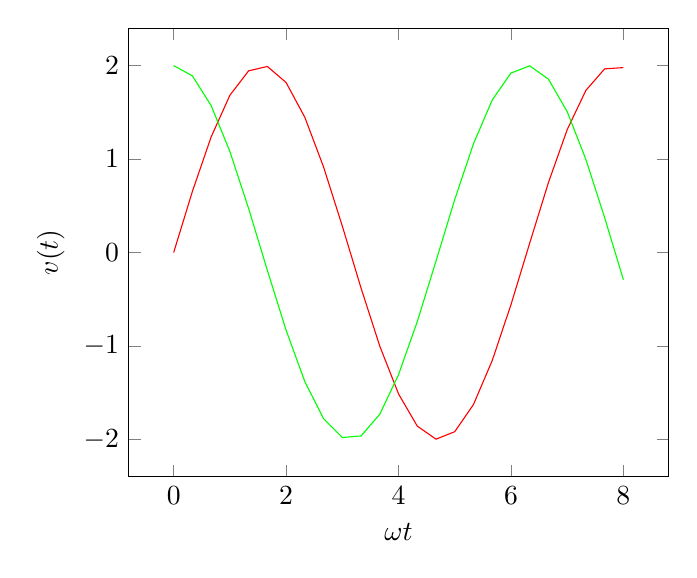
\begin{tikzpicture}
        \begin{axis}[xlabel=$\omega t$,ylabel=$v(t)$]
            \addplot[color=red][domain=0:8]{sin(x*57.296)*2};
            \addplot[color=green][domain=0:8]{cos(x*57.296)*2};
        \end{axis}
    \end{tikzpicture}
\end{center}
\begin{itemize}
    \item Two plots of sinusoidal voltages are shown with amplitude $V_m=2$. The red plot has $\alpha=0$ and the green plot has $\alpha=\frac{\pi}{2}$
    \item A common way to show the difference between two sinusoidal signal is called the \textit{Phase Lead} or \textit{Phase Lag}. 
    \begin{itemize}
        \item The green signal leads the red signal by $\frac{\pi}{2}$ (or \SI{90}{\degree}). 
        \item The red signal lags the green the signal by $\frac{\pi}{2}$ (or \SI{90}{\degree}).
    \end{itemize}
    \item Usually, only angles between $0$ to $\pi$ is used to express phase lead or phase lag of sinusoidal signals.
\end{itemize}
\begin{definition}
    \begin{itemize}
        \item The \textbf{fundamental period} of a sinusoidal signal is the smallest positive period
        \begin{equation}
            T_0=\frac{2\pi}{\omega}
        \end{equation}
        \item The \textbf{frequency} is defined as 
        \begin{equation}
            f=\frac{1}{T_0}=\frac{\omega}{2\pi}
        \end{equation}
        The unit of frequency is in \si{\per\second} or \si{\hertz}. In north america, the standard frequency is \SI{60}{\hertz} and in the rest of the world, the frequency is \SI{50}{\hertz}.
    \end{itemize}
\end{definition}

\begin{example}
    What is the phase difference between the following sinusoidal signals. 
    \begin{enumerate}
        \item \begin{align*}
            v_1(t)&=A_1\sin(\omega_1t+10\si{\degree})\\
            v_2(t)&=A_2\sin(\omega_2t+70\si{\degree})
        \end{align*}
        \item \begin{align*}
            v_1(t)&=-10\cos(\omega t+\SI{50}{\degree})\\
            v_2(t)&=12\sin(\omega t-\SI{10}{\degree})
        \end{align*}
    \end{enumerate}
\end{example}
\begin{sol}
    \begin{enumerate}
        \item We first notice that the frequency given for $v_1$ is $\omega_1$ and $v_2$ is $\omega_2$. Note that \textbf{if $\omega_1\neq\omega_2$, the phase difference is not defined for $v_1$ and $v_2$.}

        If $\omega_1=\omega_2$, the phase difference 
        \begin{equation}
            \Delta\alpha=\SI{70}{\degree}-\SI{10}{\degree}=\SI{60}{\degree}
        \end{equation}
        Since we subtracted the phase angle of $v_2$ from that of $v_1$, thus this shows $v_2$ \textbf{leads} $v_1$ by \SI{60}{\degree}.
        \begin{center}
            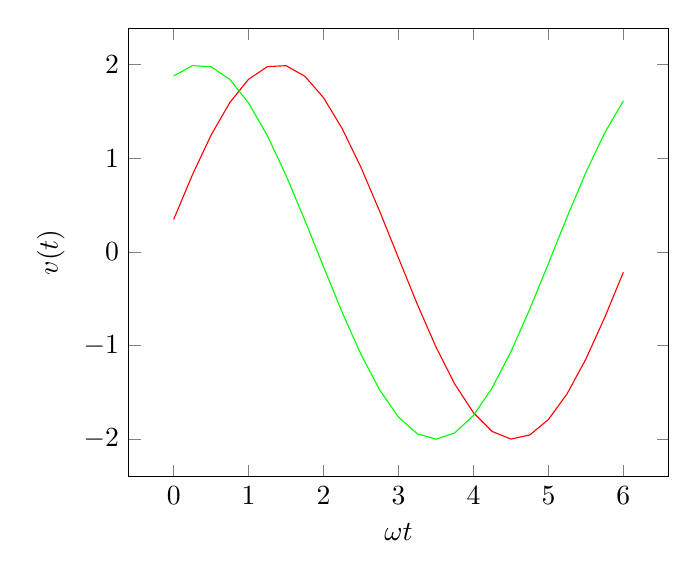
\begin{tikzpicture}
                \begin{axis}[xlabel=$\omega t$, ylabel=$v(t)$]
                    \addplot[color=red][domain=0:6]{sin(x*57.296+10)*2};
                    \addplot[color=green][domain=0:6]{sin(x*57.296+70)*2};
                \end{axis}
            \end{tikzpicture}
        \end{center}
        \item Note when comparing the phase difference between two sinusoidal signals, the trignometric function used must be the same as well as the magnitude of the ampliutude. Thus, $v_1(t)$ must be converted using the trignometric identities to 
        \begin{equation}
            v_1(t)=10\sin(\omega t-\SI{40}{\degree})
        \end{equation}
        Then, comparing that with the phase of $v_2$, 
        \begin{equation}
            \Delta\alpha=(\SI{-10}{\degree})-(\SI{-40}{\degree})=\SI{30}{\degree}
        \end{equation}
        Therefore, $v_2$ lags $v_1$ by \SI{30}{\degree}, or equivalently, $v_1$ lags $v_2$ by \SI{30}{\degree}.
    \end{enumerate}
\end{sol}
\begin{definition}
    A \textbf{Phasor} is an object used for AC circuit analysis used to describe sinusoidal signals. Take the voltage 
    \begin{equation}
        v(t)=V_m\cos(\omega t+\alpha)=\text{Re}(V_me^{j(\omega t+\alpha)})=\text{Re}(V_me^{j\alpha}e^{j\omega t})
    \end{equation}
    If the angular frequency is known, $v(t)$ can be uniquely determined using a complex number whose magnitude and angle are $V_m$ and $\alpha$ respectively. This complex number 
    \begin{equation}
        \mathbf V=V_me^{j\alpha}
    \end{equation}
    $\mathbf V$ is known as the phasor for $v(t)$. The phasor is usually denoted with an uppercase letter (also boldface in print, but just uppercase for written).
\end{definition}
\begin{itemize}
    \item Phasors are used because it is very difficult to do arithmitic on sinusoidal, but for complex number arithmitic is much simpler. 
    \item To solve an AC circuit, it is common to first transform the problem from the time domain to the phasor domain, solve it there, then transform the solution back into the time domain. 
    \item Since a phasor is determined by a magnitude and angle, they can be treated as vectors. 
\end{itemize}
\begin{example}
    Show the phasor diagram for the following AC voltage and current. Find their phase difference.
    \begin{align*}
        v(t)&=V_m\cos(377t+\SI{60}{\degree})\\
        i(t)&=I_m\sin(377t+\SI{30}{\degree})
    \end{align*}
\end{example}
\begin{sol}
    For the voltage phasor, 
    \begin{equation}
        \mathbf V=V_me^{j\SI{60}{\degree}}=V_m\angle\SI{60}{\degree}
    \end{equation}
    For the current phasor, first change the $\sin$ function to $\cos$ function using the trignometric identity. Then,
    \begin{equation}
        \mathbf I=I_me^{-j\SI{60}{\degree}}=I_m\angle\SI{-60}{\degree}
    \end{equation}
    \begin{center}
        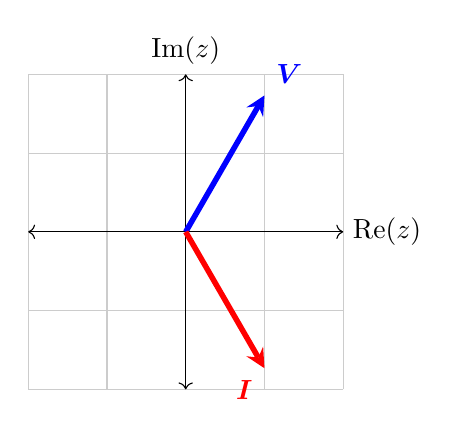
\begin{tikzpicture}
            \draw[thin,gray!40] (-2,-2) grid (2,2);
            \draw[<->] (-2,0)--(2,0) node[right]{Re$(z)$};
            \draw[<->] (0,-2)--(0,2) node[above]{Im$(z)$};
            \draw[line width=2pt,blue,-stealth](0,0)--(1,1.732) node[anchor=south west]{$\boldsymbol{V}$};
            \draw[line width=2pt,red,-stealth](0,0)--(1,-1.732) node[anchor=north east]{$\boldsymbol{I}$};
          \end{tikzpicture}
    \end{center}
\end{sol}

\begin{example}
    Using phasors, find $i_1+i_2$.
    \begin{align*}
        i_1(t)&=4\cos(\omega t+\SI{30}{\degree})\\
        i_2(t)&=5\sin(\omega t-\SI{20}{\degree})
    \end{align*}
\end{example}
\begin{sol}
    First convert these into phasors. Note to use the trignometric identity for $i_2$ to obtain
    \begin{align*}
        \mathbf I_1&=4\angle\SI{30}{\degree}\\
        \mathbf I_2&=5\angle\SI{-110}{\degree}
    \end{align*}
    Add in the rectangular form, 
    \begin{equation}
        \begin{aligned}
            \mathbf I_1+\mathbf I_2&=4\angle\SI{30}{\degree}+5\angle\SI{-110}{\degree}\\
            &=4\cos(\SI{30}{\degree})+j4\sin(\SI{30}{\degree})+5\cos(\SI{-110}{\degree})+j5\cos(\SI{-110}{\degree})\\
            &=1.754+j2.698\\
            &=3.218\angle \SI{-56.98}{\degree}
        \end{aligned}
    \end{equation}
    The sum of the two signals is then 
    \begin{equation}
        i_1+i_2=3.218\cos(\omega t-\SI{56.98}{\degree})
    \end{equation}
\end{sol}

\subsection{Calculus with Phasors}
\begin{proposition}
    For a phasor $\mathbf Z$,
    \begin{align}
        \dot{\mathbf Z}&=j\omega\mathbf Z\\
        \int \mathbf Z\, \dd t&=\frac{\mathbf Z}{j\omega}
    \end{align}
\end{proposition}
\begin{prooof}
    Take the phasor $\mathbf{V}=V_m\angle\phi=V_m e^{j\phi}$. Take the derivative of what the phasor represents
    \begin{align}
        v(t)&=V_m\cos(\omega t+\phi)\\
        \dot v(t)&=-V_m\omega\sin(\omega t+\phi)=+V_m\omega\cos(\omega t+\phi+\SI{90}{\degree})
    \end{align}
    The phasor for $\dot v(t)$ is
    \begin{equation}
        \dot{\mathbf{V}}=V_m\omega e^{\omega t}e^{j\phi}e^{j\SI{90}{\degree}}=j\omega (V_me^{j\phi})=j\omega\mathbf V
    \end{equation} 

    Taking the integral of what the phasor represent,
    \begin{equation}
        \int v(t)\dd t=\frac{V_m}{\omega}\sin(\omega t+\phi)=\frac{V_m}{\omega}\cos(\omega t+\phi-\SI{90}{\degree})
    \end{equation}
    For the phasor, 
    \begin{equation}
        \int \mathbf{V}\dd t=\frac{V_m}{\omega}e^{j(\phi-\SI{90}{\degree})}=\frac{1}{j\omega}(V_me^{j\phi})=\frac{\mathbf V}{j\omega}
    \end{equation}
\end{prooof}

\subsection{Phasor relation for the voltage and current of R, L, and C}
\begin{itemize}
    \item For a resistor, consider the current through a resistor $\mathbf I=I_m\angle\alpha$. Applying Ohm's law, 
    \begin{equation}
        \mathbf V=RI_m\angle \alpha=R\mathbf I
    \end{equation}
    \begin{center}
        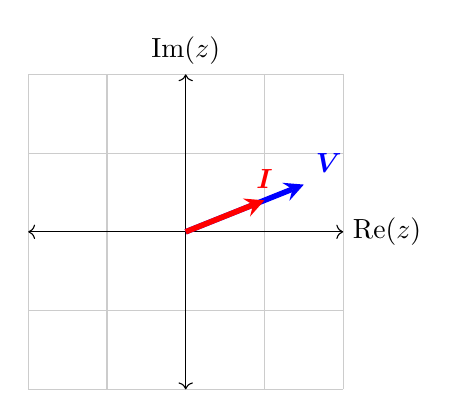
\begin{tikzpicture}
            \draw[thin,gray!40] (-2,-2) grid (2,2);
            \draw[<->] (-2,0)--(2,0) node[right]{Re$(z)$};
            \draw[<->] (0,-2)--(0,2) node[above]{Im$(z)$};
            \draw[line width=2pt,blue,-stealth](0,0)--(1.5,0.6) node[anchor=south west]{$\boldsymbol{V}$};
            \draw[line width=2pt,red,-stealth](0,0)--(1,0.4) node[anchor=south]{$\boldsymbol{I}$};
          \end{tikzpicture}
    \end{center}
    \item For an inductor, consider the current phasor in the inductor as $\mathbf I=I_m\angle\alpha$. It is known that $v(t)=L\dot i$, thus 
    \begin{equation}
        \mathbf V=j\omega L\mathbf I
    \end{equation}
    \begin{center}
        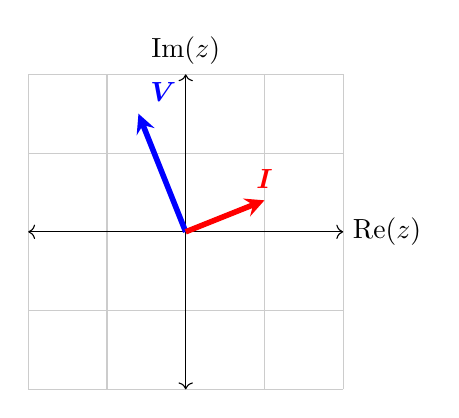
\begin{tikzpicture}
            \draw[thin,gray!40] (-2,-2) grid (2,2);
            \draw[<->] (-2,0)--(2,0) node[right]{Re$(z)$};
            \draw[<->] (0,-2)--(0,2) node[above]{Im$(z)$};
            \draw[line width=2pt,blue,-stealth](0,0)--(-0.6,1.5) node[anchor=south west]{$\boldsymbol{V}$};
            \draw[line width=2pt,red,-stealth](0,0)--(1,0.4) node[anchor=south]{$\boldsymbol{I}$};
          \end{tikzpicture}
    \end{center}
    \item For a capacitor, consider the voltage phasor in the capacitor as $\mathbf V=V_m\angle\alpha$. It is known that $i(t)=C\dot v$,
    \begin{equation}
        \mathbf V=\frac{\mathbf I}{j\omega C}
    \end{equation}
    \begin{center}
        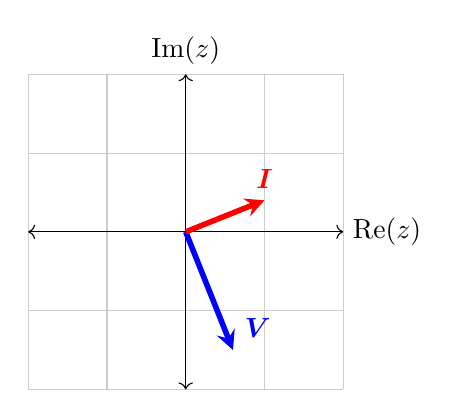
\begin{tikzpicture}
            \draw[thin,gray!40] (-2,-2) grid (2,2);
            \draw[<->] (-2,0)--(2,0) node[right]{Re$(z)$};
            \draw[<->] (0,-2)--(0,2) node[above]{Im$(z)$};
            \draw[line width=2pt,blue,-stealth](0,0)--(0.6,-1.5) node[anchor=south west]{$\boldsymbol{V}$};
            \draw[line width=2pt,red,-stealth](0,0)--(1,0.4) node[anchor=south]{$\boldsymbol{I}$};
          \end{tikzpicture}
    \end{center}
\end{itemize}
\subsection{KVL and KCL the phasor domain}
\begin{proposition}
    Suppose there is a loop in the circuit of $N$ circuit elements with voltage phasors $\mathbf V_1,\mathbf V_2,\dots,\mathbf{V_N}$ with the same (angluar) frequency $\omega$. Then, KVL for phasors requires 
    \begin{equation}
        \sum\mathbf V_n=\mathbf V_1+\mathbf V_2+\dots \mathbf V_N=0
    \end{equation}
\end{proposition}
\begin{proposition}
    Suppose a node with $N$ current paths and incoming current phasors $\mathbf I_1,\mathbf I_2,\dots,\mathbf{I_N}$ with the same (angluar) frequency $\omega$. Then, KCL for phasors requires
    \begin{equation}
        \sum \mathbf I_n=\mathbf I_1+\mathbf I_2+\dots \mathbf I_N=0
    \end{equation}
\end{proposition}
\section{Impedence}
\begin{definition}
    Take an arbiturary circuit element with a sinusoidal voltage and current with the same frequency. The voltage and current phasors are $\mathbf V$ and $\mathbf I$ respectively. Then,
    \begin{equation}
        Z\equiv\frac{\mathbf V}{\mathbf I}=\frac{V_m\angle\theta_v}{I_m\angle\theta_i}=\frac{V_m}{I_m}\angle(\theta_v-\theta_i)
    \end{equation}
    Rewriting the impedence in rectangular form, 
    \begin{equation}
        Z\equiv R+jX
    \end{equation}

    \begin{itemize}
        \item The real part of the impedence $R$ is called \textit{resistance}. 
        \item The imaginary part of impedence $X$ is called \textit{reactance}. 
        \item The units for $Z,R,X$ is Ohm.
        \item \textbf{Note} if the passive sign convention does not hold for $\mathbf V$ and $\mathbf I$, then $Z=-\mathbf V/\mathbf I$.
    \end{itemize}

    \begin{equation}
        \det(\lambda \mathbbm{1}_{n\times n})=\lambda^n
    \end{equation}
\end{definition}
\begin{itemize}
    \item For DC circuits there is resistance and conductance. For AC circuits,
\end{itemize}
\begin{definition}
    The admittance of an circuit element is with current phasor $\mathbf{I}$ and voltage phasor $\mathbf{V}$ is 
    \begin{equation}
        Y\equiv\frac{\mathbf I}{\mathbf V}=\frac{I_m}{V_m}\angle(\theta_i-\theta_v)
    \end{equation}
    Rewriting this in the rectangular form, 
    \begin{equation}
        Y=G+jB
    \end{equation}
    \begin{itemize}
        \item The real part of the admittance $G$ is called \textit{conductance}.
        \item The imaginary part of the admittance $B$ is called
    \end{itemize}
\end{definition}

\subsection{Series and parellel connected impedances}
\begin{proposition}
    \begin{itemize}
        \item The equivalent impedance of multiple circuit elements connected in series and parellel behaves the same as the resistance in DC circuits. 
        \item The equivalent admittance for multiple circuit elements connected in parellel behaves the same as conductance in DC circuits.
    \end{itemize}
\end{proposition}

\subsection{The impedance for the resistor, inductor, and capacitor}
\begin{itemize}
    \item For a resistor,
    \begin{equation}
        Z_R=\frac{\mathbf{V}}{\mathbf{I}}=\frac{R\mathbf I}{\mathbf I}=R
    \end{equation}
    \item The impedance of a resistor is the resistance itself lmao. In the complex plane, this is a positive real number.
    \item For an inductor,
    \begin{equation}
        Z_L=\frac{\mathbf V}{\mathbf I}=\frac{j\omega L\mathbf I}{\mathbf I}=j\omega L    
    \end{equation}
    \item In the complex plane, the impedance of an inductor is on the positive imaginary axis.
    \item Note that for the same inductor, the impedance is also dependent on the frequency of the circuit. 
    \item In the limit where $\omega\to 0$, the impedance approaches 0, which is the reason that under steady state DC conditions, an inductor behaves like a short circuit.
    \item For a capacitor, 
    \begin{equation}
        Z_C=\frac{\mathbf V}{\mathbf I}=\frac{\frac{-j}{\omega C}\mathbf I}{\mathbf I}=\frac{-j}{\omega C}=\frac{1}{\omega C}
    \end{equation}
    \item In the complex plane, the impedance of a capacitor is on the negative imaginary axis.
\end{itemize}

\subsection{The impedance of RL, RC, LC, and RLC circuits}
\subsubsection{RL Circuit}
\begin{center}
    \begin{circuitikz}
        \draw (0,0)node[left]{b}
        to (2,0)
        to[L=$L$](2,2)
        to[R=$R$] (2,4)
        to(0,4)node[left]{a};
    \end{circuitikz}
\end{center}
\begin{equation}
    Z_{RL}=Z_R+Z_L=R+j\omega L
\end{equation}
\begin{itemize}
    \item $Z_{RL}$ is located in the first quadrant of the complex plane. The angle of the impedance is 
    \begin{equation}
        \angle Z_{RL}=\arctan(\frac{\omega L}{R})
    \end{equation}
    \item If $Z_R>>Z_L\iff R>>\omega L\implies\angle Z_{RL}\to\SI{0}{\degree}$
    \item If $Z_R<<Z_L\iff R<<\omega L\implies\angle Z_{RL}\to\SI{90}{\degree}$
    \item Because of this, the voltage of an RL circuit leads the current by an angle between \SI{0}{\degree} to \SI{90}{\degree}
    \begin{equation}
        Z_{RL}=\frac{V_m}{I_m}\angle(\theta_v-\theta_i)\implies \SI{0}{\degree}<\theta_v-\theta_i<\SI{90}{\degree}
    \end{equation}
    \item In the time domain, the voltage will lead the current by a quarter of a period. (blue is voltage, red is current)
    \begin{center}
        \begin{tikzpicture}
            \begin{axis}[xlabel=$\omega t$]
                \addplot[domain=0:5][color=red]{sin(x*57)};
                \addplot[domain=0:5][color=blue]{sin(x*57+20)*0.7};
            \end{axis}
        \end{tikzpicture}
    \end{center}
\end{itemize}
\subsubsection{RC Circuit}
\begin{center}
    \begin{circuitikz}
        \draw (0,0)node[left]{b}
        to (2,0)
        to[C=$C$](2,2)
        to[R=$R$] (2,4)
        to(0,4)node[left]{a};
    \end{circuitikz}
\end{center}
\begin{equation}
    Z_{RC}=Z_R+Z_C=R-\frac{j}{\omega C}
\end{equation}
\begin{itemize}
    \item $Z_{RC}$ is located in the fourth quadrant of the complex plane. The angle of the impedance is 
    \begin{equation}
        \angle Z_{RC}=\arctan(-\frac{1}{\omega RC})
    \end{equation}
    \item If $R>>\frac{1}{\omega C}\implies\angle Z_{RC}\to \SI{0}{\degree}$
    \item If $R<<\frac{1}{\omega C}\implies\angle Z_{RC}\to \SI{-90}{\degree}$
    \item $\SI{-90}{\degree} < \theta_v-\theta_i < \SI{0}{\degree}$,
    \item Because of this, the voltage of an RC circuit lags the current by an angle between \SI{0}{\degree} to \SI{90}{\degree}.
\end{itemize}
\subsubsection{LC Circuit}
\begin{center}
    \begin{circuitikz}
        \draw (0,0)node[left]{b}
        to (2,0)
        to[C=$C$](2,2)
        to[L=$L$] (2,4)
        to(0,4)node[left]{a};
    \end{circuitikz}
\end{center}
\begin{equation}
    Z_{LC}=Z_L+Z_C=j\omega L-\frac{j}{\omega c}=j\left(\omega L-\frac{1}{\omega C}\right)
\end{equation}
\begin{itemize}
    \item The impedance is purely imaginary. 
    \item If $\omega L>\frac{1}{\omega C}$, the impedance will be on the positive imaginary axis. These circuit are called \textbf{inductive} LC circuits.
    \item If $\omega L<\frac{1}{\omega C}$, the impedance will be on the negative imaginary axis. These circuit are called \textbf{capacitive} LC circuits.
    \item The voltage can either lead or lag the current, depending on the if it is an inductive or capacitive circuit. 
\end{itemize}
\subsubsection{RLC Circuit}
\begin{center}
    \begin{circuitikz}
        \draw (0,0)node[left]{b}
        to (2,0)
        to[C=$C$](2,1.3)
        to[L=$L$] (2,2.7)
        to[R=$R$] (2,4)
        to(0,4)node[left]{a};
    \end{circuitikz}
\end{center}
\begin{equation}
    Z_{RLC}=Z_R+Z_L+Z_C=R+j\left(\omega L-\frac{1}{\omega C}\right)
\end{equation}
\begin{itemize}
    \item The real part of the impedance is positive, but the imaginary part can be either positive or negative. Thus, the complex number can be located in first or fourth quadrant of the complex plane.
    \item If $Z_{RLC}$ is in the first quadrant ($\omega L>\frac{1}{\omega C}$), the RLC circuit is called an \textbf{inductive} (RL) circuit.
    \item If \(Z_{RLC}\) is in the fourth quadrant ($\omega_L <\frac{1}{\omega C}$), the RLC circuit is called an \textbf{capacitive} (RC) circuit. 
\end{itemize}
\begin{example}
    How do RL, RC, LC, and RLC circuits behave if they are connected in parellel?
\end{example}
% mouse hover event
% get mouse position (system.windows.form.cursor.positon)
% Form.location (where the form is on the screen)
% click action (for the form)

% image box
% C# bitmap for updating image
\section{Analysis of AC Circuits}
\begin{itemize}
    \item Application of KVL and KCL in the phasor domain
    \item The function of $Z=\mathbf{V}/\mathbf{I}$ relation in AC circuit analysis is similar to the function of $R=v/i$ in DC circuit analysis.
    \item All the circuit analysis techniques for DC circuits (nodal analysis, mesh analysis, voltage division, superposition, etc) are applicable to AC circuits as well. The only difference is that complex numbers must be used (phasors and impedances)
\end{itemize}

\begin{example}
    \begin{center}
        \begin{circuitikz}
            \draw (0,3)
            to[V=$v(t)$] (0,0)
            to(6,0)
            to[R=\SI{8}{\ohm}](6,3)
            to[L=\SI{0.2}{H}](3,3)
            to[C=\SI{2}{mF},i<=$i(t)$](0,3);
            \draw(3,3)
            to[R=\SI{3}{\ohm}](3,1.2)
            to[C=\SI{10}{mF}](3,0);
        \end{circuitikz}
    \end{center}
    $v(t)=20\cos(50t)$. Find $i(t)$.
\end{example}
\begin{sol}
    First we must convert all voltage and current to phasors, and all the circuit elements to impedances. The voltage source has a voltage phasor $\mathbf V=20\angle 0$.

    To find the impedances, we call the impedance of the \SI{2}{mF} capacitor $Z_1$, the RC component $Z_2$ and the RL component $Z_3$. The frequency of the circuit is dependent on the source, which here is $\omega=50$
    \begin{align}
        Z_1&=\frac{-j}{\omega C_1}=\frac{-j}{50\times 0.002}=-j\SI{10}{\ohm}\\
        Z_2&=R_2-\frac{j}{\omega C_2}=3-\frac{j}{50\times 0.01}=3-j2\si{\ohm}\\
        Z_3&=R_3+j\omega L_2=8+j50\times 0.2=8+j10\si{\ohm}
    \end{align}
    Representing the circuit in the phasor domain,
    \begin{center}
        \begin{circuitikz}
            (0,3)
            to[V=20$\angle$0] (0,0)
            to(6,0)
            to[R=\SI{8}{\ohm}](6,3)
            to[L=\SI{0.2}{H}](3,3)
            to[C=\SI{2}{mF},i<=$i(t)$](0,3);
            \draw(3,3)
            to[R=\SI{3}{\ohm}](3,1.2)
            to[C=\SI{10}{mF}](3,0);
        \end{circuitikz}
    \end{center}
    We can find the equivalent impedance, note $Z_2$ and $Z_3$ is connected in parellel, which is connected in series with $Z_1$. Thus, 
    \begin{equation}
        Z_{eq}=Z_1+Z_2||Z_3=Z_1+\frac{Z_2Z_3}{Z_2+Z_3}=3.22+j11.07\si{\ohm}=11.53\angle \SI{-73.5}{\ohm}
    \end{equation}
    Now using ohm's law for phasors,
    \begin{equation}
        \mathbf I=\frac{\mathbf V}{Z_{eq}}=\frac{20\angle 0}{11.53\angle -73.5\si{\degree}}=1.73\angle 73.5\si{\degree}
    \end{equation}
    Converting this back to the time domain, 
    \begin{equation}
        i(t)=1.73\cos(50t+\SI{73.5}{\degree})
    \end{equation}
\end{sol}
\begin{itemize}
    \item Note that this circuit can be replaced with an equivalent RL or RC.
    \item If the reactance is positive, it can be replaced with RL, otherwise it can be replaced with RC. (Note this is possible because the frequency remains constant)
    \item In the example above, $R_{eq}=\SI{3.22}{\ohm}, C_{eq}=\SI{1.81}{mF}$.
\end{itemize}


\end{document}